\documentclass[a4paper,10pt]{article}

\usepackage{ucs}
\usepackage[utf8]{inputenc}
\usepackage{babel}
\usepackage{fontenc}
\usepackage{graphicx}

\usepackage[dvips]{hyperref}
\usepackage{tikz}
\date{}

\usetikzlibrary{patterns}
\newcommand{\anneau}[2]%
{\fill[#2,even odd rule] (#1) circle (2.5) circle (3);}

\newcommand{\recouvrement}[3]%
{\fill[#3] (#1) ++(#2:3)
arc (#2:{#2-30}:3) -- ++({#2-30}:-0.5)
arc ({#2-30}:#2:2.5) -- cycle;}

\newcommand{\rect}[4]{\draw (#1, #2)--(#1+#3,#2+#4)--(#1+#3,#2+#4);}

\title{101 Tikz Examples}

\author{}

\begin{document}
\maketitle




\section{Thales }

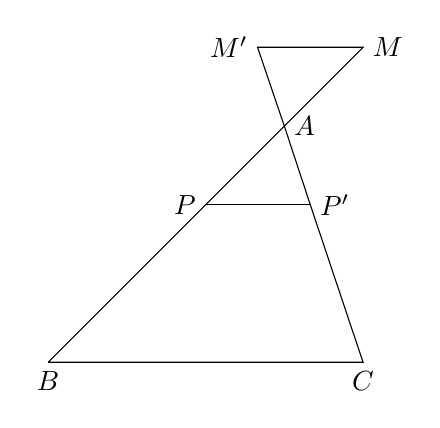
\begin{tikzpicture} 
 \draw (0,0)node[below]{$B$}--(4,0)node[below]{$C$}--(3.33,2)node[right]{$P'$}--(3,3)node[right]{$A$}
 --(2.66,4)node[left]{$M'$}--(4,4)node[right]{$M$}--(2,2)node[left]{$P$}--(0,0);
 \draw (2,2)--(3.33,2);
 \end{tikzpicture}
 
 
 \section{Graph of function $f(x)=(x-2)^2-2$} 
 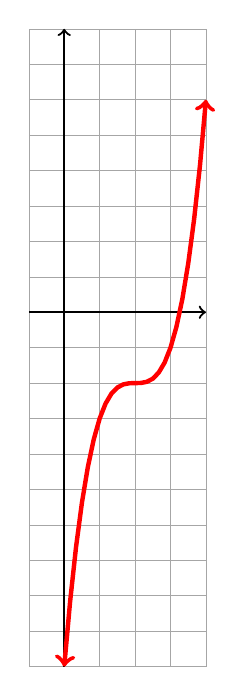
\begin{tikzpicture}
 \begin{scope}[scale=.45]
\draw[help lines, gray!70] (-1,-10) grid (4,8);
\draw[thick,->] (-1,0)--(4,0);
	\draw[thick,->] (0,-10)--(0,8);
%\draw [re,very thick] (-4,-4) to (4,4);
\draw[red, ultra thick, domain=0:4,<->] plot (\x, {(\x-2)*(\x-2)*(\x-2)-2});
\end{scope}		
\end{tikzpicture}


 \section{Straddle/Strangle} 
 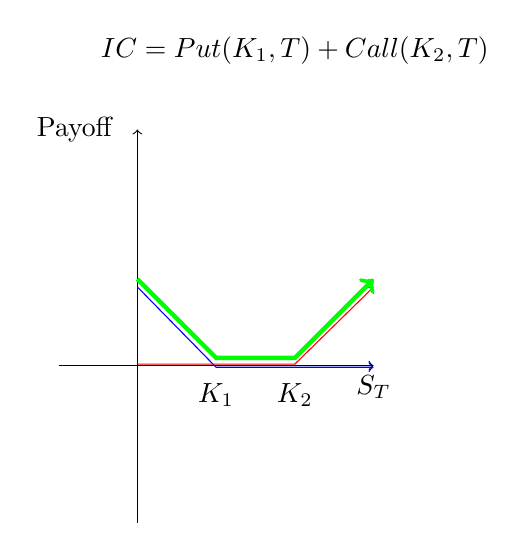
\begin{tikzpicture}
\draw[->]  (-1,0)--(3,0);
\draw[->] (0,-2)--(0,3);
\draw [ blue,->] (0,1)--(1.,-0.02)--(3 ,-.02);
\draw [ red,->] (0,.02)--(2.,0.02)--(3 ,1);
\draw [ultra thick,green,->] (0,1.1)-- (1  ,.1)--(2,.1)--(3,1.1);
\node [below] at (3,0) {$ S_T $};
\node [left] at (-0.2,3) {Payoff};
\node [below] at (1.,-.10) {$ K_1$};
\node [below] at (2.,-.10) {$ K_2$};
%\node[right,below] at (2,2) {$m=1$};
\node at (2,4) {$ IC=Put(K_1,T)+Call(K_2,T) $};
\end{tikzpicture}

 \section{A graph with in and out} 
 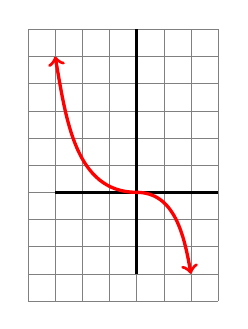
\begin{tikzpicture}	
\begin{scope}[scale=.345]
\draw[help lines] (-4,-4) grid (3,6);
\draw [very thick](-3,0)--(3,0);
	\draw[very thick] (0,-3)--(0,6);
\draw [red,very thick,<->] (-3,5) to [out=-80, in=180](0,0)  to [out=0,in=100](2,-3);
	\end{scope}		
\end{tikzpicture}


 \section{Graph $f(x)=\frac1x$} 
 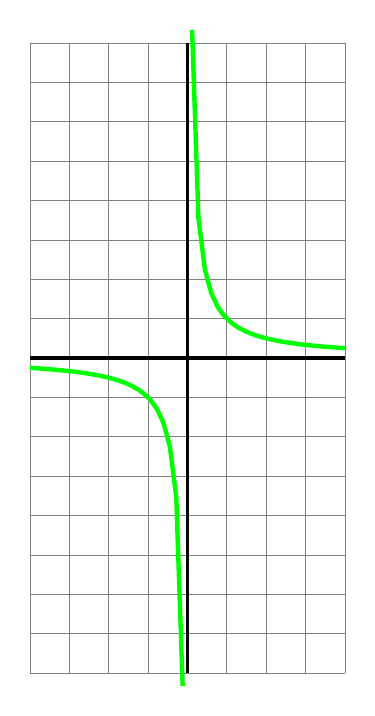
\begin{tikzpicture}	
\begin{scope}[scale=.5]
\draw[help lines] (-4,-8) grid (4,8);
\draw[very thick] (-4,0)--(4,0);
\draw[very thick] (0,-8)--(0,8);
%\draw [red,very thick] (-4,4) to(0,0) to (4,4);
\draw[green, ultra thick, domain=0.12:4] plot (\x, {1/\x});
\draw[green, ultra thick, domain=0.12:4] plot (-\x, {-1/\x});
	\end{scope}		
\end{tikzpicture}

 \section{Random curve} 
 
 
 \begin{tikzpicture}	
\begin{scope}[scale=.5]
\draw (0,0) to [in=200,out=0](2,3) to [out=20] (4,1);
	\end{scope}		
\end{tikzpicture}






 \section{Orthocenter } 
 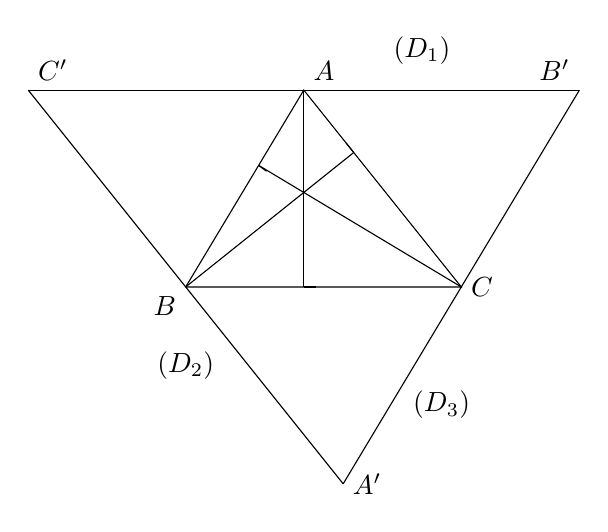
\begin{tikzpicture}[scale=0.5]
%\draw[help lines](-3,-2)grid(8,5);
%\draw[step=1cm,gray,very thin] (-7.9,-7.9) grid (10.9,10.9);
\draw (0,0)node[below left]{$B$}--(7,0)node[ right]{$C$}--(3,5)node[above right]{$A$}--(0,0);
\draw (0.0, 0.0)--(4.268, 3.415);
\draw (7.0, 0.0)-- (1.853, 3.088);
\draw (3.0, 5.0)-- (3.0, 0.0);
%\draw (7,0)--++(3,5)--++(-6,-10);
\draw (7,0)--(10,5)--(4,-5);
\draw(0,0)--(-4,5)--(4,-5);
\draw (10,5)--(-4,5);
\rect 3 0 {0.3}{0}
\rect{4.268}{3.415}{-.2}{0.25}
\rect{1.853}{3.088}{.2}{-0.15}
\node[above left] at (10,5){$B'$};
\node[right] at (4,-5){$A'$};
\node[above right] at (-4,5){$C'$};
\node at (6,6){$(D_1)$};
\node at (0,-2){$(D_2)$};
\node at (6.5,-3){$(D_3)$};
\end{tikzpicture}


 
\section{Random curve} 
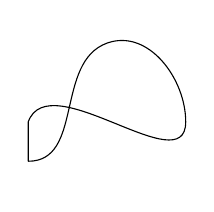
\begin{tikzpicture}	
\begin{scope}[scale=.5]
\draw (0,0) to [in=200,out=0](2,3) to [out=20,in=90] (4,1) to [out=270,in=70](0,1) to (0,0);
	\end{scope}		
\end{tikzpicture}


 \section{Curve $f(x)=x^2$} 
 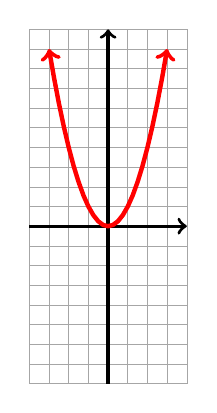
\begin{tikzpicture}
\begin{scope}[scale=.25]
\draw[help lines, gray!70] (-4,-8) grid (4,10);
\draw[very thick,->] (-4,0)--(4,0);
	\draw[very thick,->] (0,-8)--(0,10);
%\draw [red,very thick] (-4,-4) to (4,4);
\draw[red, <->,ultra thick, domain=-3:3] plot (\x, {\x*\x});
	\end{scope}		
\end{tikzpicture}





 \section{A graph with dots} 
 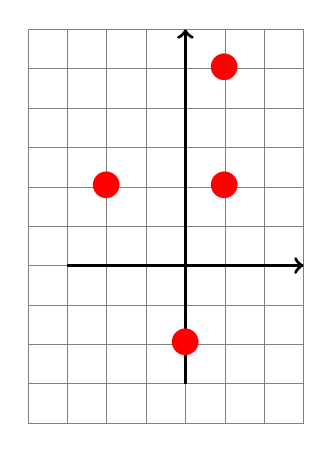
\begin{tikzpicture}	
\begin{scope}[scale=.5]
\draw[help lines] (-4,-4) grid (3,6);
\draw[very thick,->] (-3,0)--(3,0);
	\draw[very thick,->] (0,-3)--(0,6);
\draw [red,thick] (1,2)node{\begin{Huge}$\bullet$\end{Huge}};
\draw [red,thick] (1,5)node{\begin{Huge}$\bullet$\end{Huge}};
\draw [red,thick] (-2,2)node{\begin{Huge}$\bullet$\end{Huge}};
\draw [red,thick] (0,-2)node{\begin{Huge}$\bullet$\end{Huge}};
	\end{scope}		
\end{tikzpicture}




















 \section{graph $f(x)=.07x^3$} 
 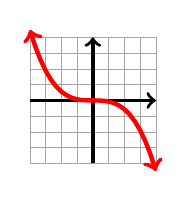
\begin{tikzpicture}
\begin{scope}[scale=.2]
\draw[help lines, gray!70] (-4,-4) grid (4,4);
\draw[very thick,->] (-4,0)--(4,0);
	\draw[very thick,->] (0,-4)--(0,4);
\draw[red, <->,ultra thick, domain=-4:4] plot (\x, {-0.07*\x*\x*\x}); 
	\end{scope}		
\end{tikzpicture}


 \section{Segment} 
 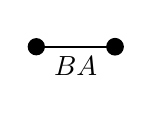
\begin{tikzpicture}	
\begin{scope}[scale=.5]
\draw[thick] (-2,0)-- (0,0);
\draw (-1,0)node[below]{$ BA $};
\draw[fill] (-0.,0) circle(.21051);
\draw[fill] (-2,0) circle(.2051);
\draw (-1,.25)node{};
	\end{scope}		
\end{tikzpicture}


 \section{Gradient} 
 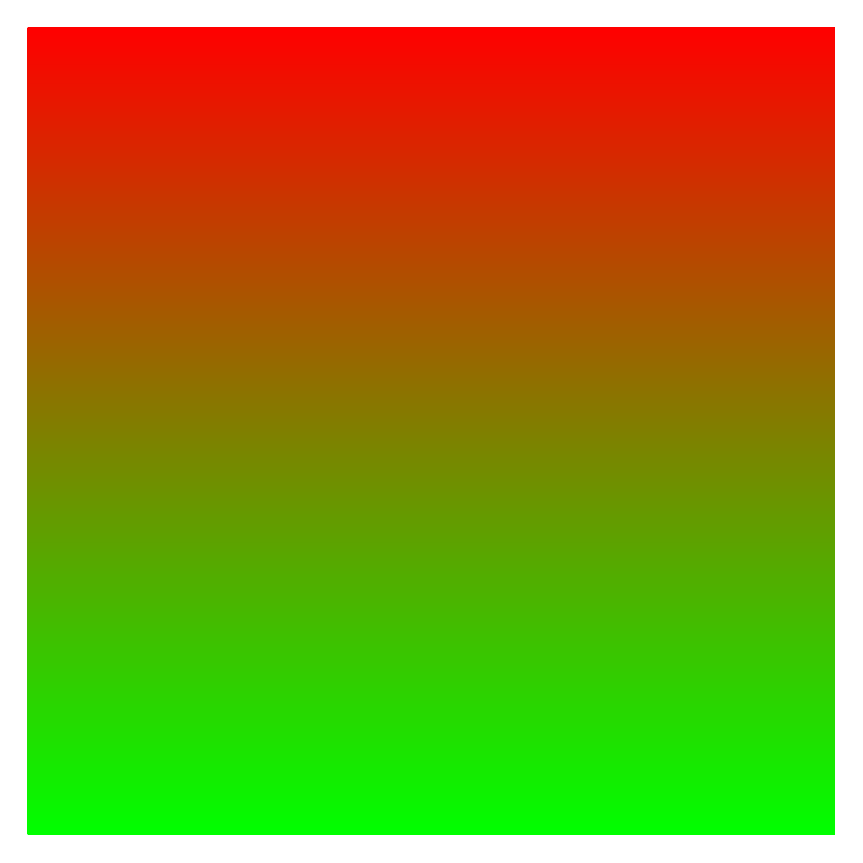
\begin{tikzpicture}[scale=.25]
\shade[top color=red, bottom color=green]
(-12,-12) rectangle (29cm,29cm);
\end{tikzpicture}

 \section{Cube} 
 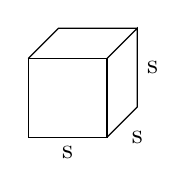
\begin{tikzpicture}
	\draw (0,0,0)--(1,0,0)--(1,1,0)--(0,1,0)--(0,0,0);
	\draw (1,1,0)--(1,1,-1)--(1,0,-1)--(1,0,0);
	\draw (0,1,0)--(0,1,-1)--(1,1,-1);
	\draw (.5,0,0) node[below]{s};
	\draw (1,0,-.5) node[below right]{s};
	\draw (1,.5,-1) node[right]{s};
\end{tikzpicture}


 \section{Area, circle, rectangle} 
 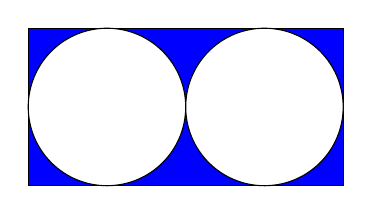
\begin{tikzpicture}
\draw[fill=blue] (-2,-1)--(2,-1)--(2,1)--(-2,1)--(-2,-1);
	\draw[fill=white] (-1,0) circle(1);
	\draw[fill=white] (1,0) circle(1);
\end{tikzpicture}


 \section{Regular triangulation} 
 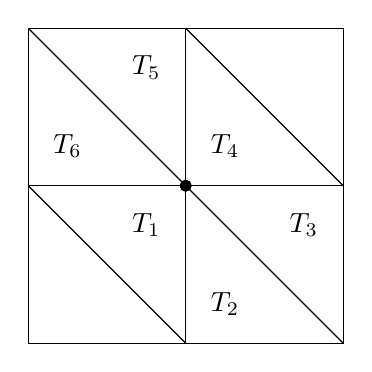
\begin{tikzpicture}
 \draw (0,0)--(4,0)--(4,4)--(0,4)--(0,0);
 \draw (0,2)--(4,2);
 \draw (2,0)--(2,4);
 \draw (0,2)--(2,0);
 \draw (2,4)--(4,2);
 \draw (0,4)--(4,0);
 \filldraw[black] (2,2) circle (2pt);
 %\draw (.5,.5) node  {$T_1$};
 \draw (1.5,1.5) node  {$T_1$};
 \draw (2.5,.5) node  {$T_2$};
 \draw (3.5,1.5) node  {$T_3$};
 \draw (.5,2.5) node  {$T_6$};
 \draw (1.5,3.5) node  {$T_5$};
 \draw (2.5,2.5) node  {$T_4$};
% \draw (3.5,3.5) node  {$T_8$};
\end{tikzpicture}


 \section{A sequence} 
 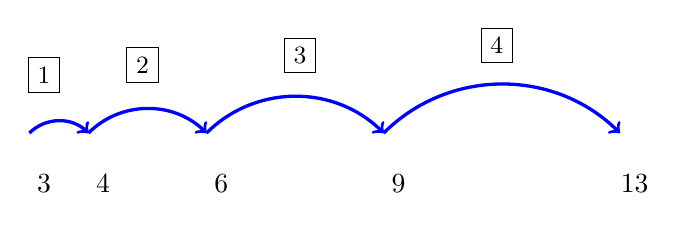
\begin{tikzpicture}[scale=.5]
\begin{scope}[scale=1.5]
    \draw(3,0) node{$3$};
     \draw(4,0) node{$4$};
 \draw[->,very thick,blue](3-.25,0.85) to[out=45,in=135] (4-.25,.85);
      \draw(6,0) node{$6$};
 \draw[->,very thick,blue](4-.25,0.85) to[out=45,in=135] (6-.25,.85);
      \draw(9,0) node{$9$};
 \draw[->,very thick,blue](6-.25,0.85) to[out=45,in=135] (9-.25,.85);
\draw(13,0) node{$13$};
 \draw[->,very thick,blue](9-.25,0.85) to[out=45,in=135] (13-.25,.85);	
\end{scope}
 
 \draw (4.5,2.75) node[draw]{\small{$1$}};
  
 \draw (7,3) node[draw]{\small{$2$}};
  
 \draw (11,3.25) node[draw]{\small{$3$}};
  
 \draw (16,3.5) node[draw]{\small{$4$}};
    \end{tikzpicture}
    
    
    
 \section{Graph $f(x)=-\frac1x$} 
 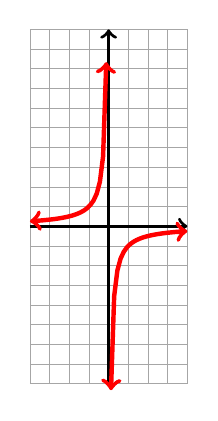
\begin{tikzpicture}
\begin{scope}[scale=.25]
\draw[help lines, gray!70] (-4,-8) grid (4,10);
\draw[very thick,->] (-4,0)--(4,0);
	\draw[very thick,->] (0,-8)--(0,10);
%\draw [red,very thick] (-4,-4) to (4,4);
\draw[red, <->,ultra thick, domain=-4:-.12] plot (\x, {-1/(\x )});
\draw[red, <->,ultra thick, domain=.12:4] plot (\x, {-1/(\x )});
	\end{scope}		
\end{tikzpicture}


 \section{Graph $f(x)=\sqrt{x}$} 
 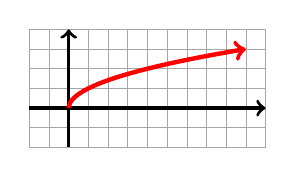
\begin{tikzpicture}
\begin{scope}[scale=.25]
\draw[help lines, gray!70] (-2,-2) grid (10,4);
\draw[very thick,->] (-2,0)--(10,0);
	\draw[very thick,->] (0,-2)--(0,4);
%\draw [red,very thick] (-4,-4) to (4,4);
\draw[red, ->,ultra thick, domain=0:3] plot (\x*\x, {\x});
	\end{scope}		
\end{tikzpicture}


 \section{A grid} 
 \newcommand{\rectz}[4]{\draw (#1, #2) rectangle  (#3,#4);}
 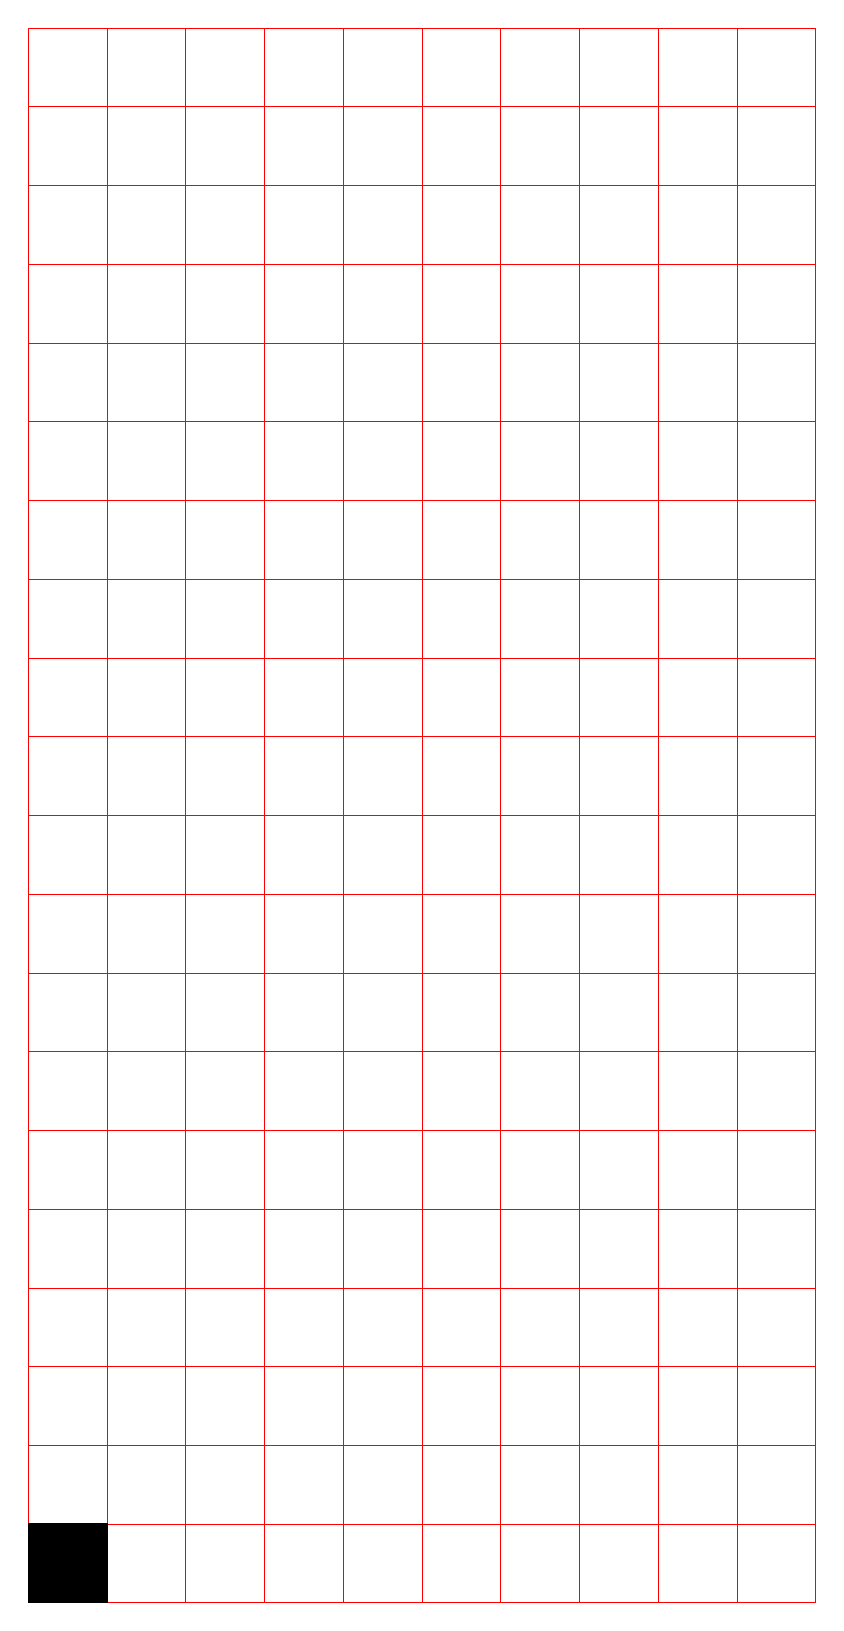
\begin{tikzpicture}
\draw[help lines ,red] (0,0) grid (10,20);%thick
\draw [fill] (0,0) rectangle (1,1);
\rectz 2 3 3 4;
\rectz 2 8 3 9;
\rectz 6 8 7 {12};
\rectz 9 {10} {10} {11};
\rectz 8 {15} {10} {16};
\end{tikzpicture}




 \section{Graph given points} 
 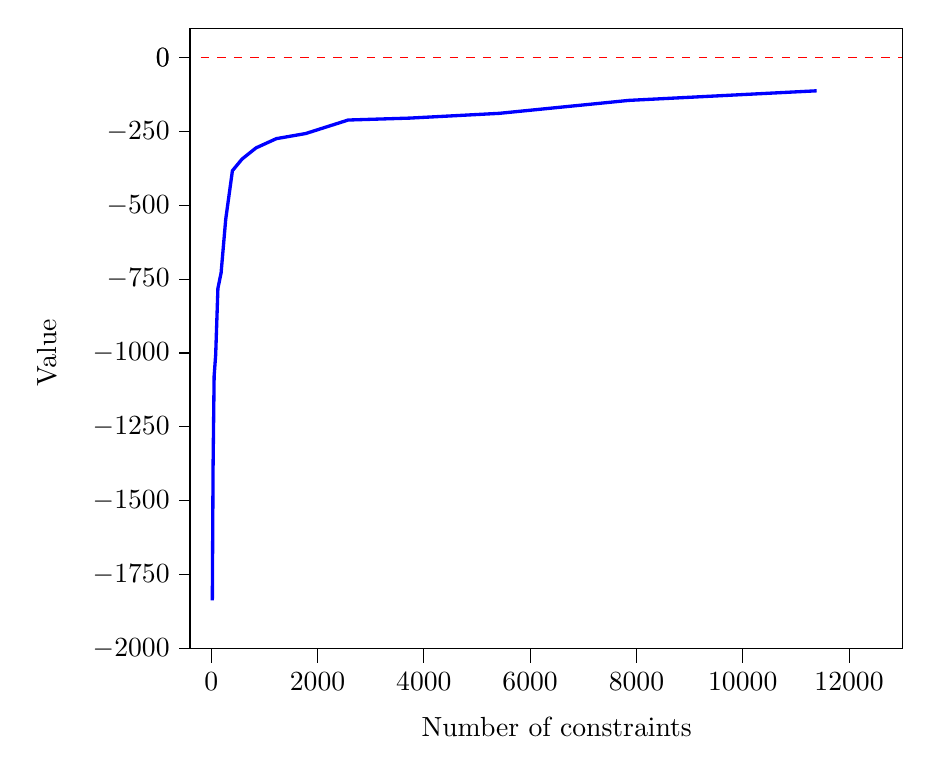
\begin{tikzpicture}[yscale=.5,xscale=.9]
 \begin{scope}[scale=.75]
\draw [very thick, blue] (0.02,-18.373506830617785)--(0.034,-13.8463936338521)--(0.054,-10.782155090319229)--(0.083,-10.059238679779357)--(0.125,-7.809713703513674)--(0.185,-7.283882026080817)--(0.272,-5.468931498801182)--(0.398,-3.8256503381170415)--(0.58,-3.4291148600527053)--(0.843,-3.052066205417267)--(1.224,-2.7399955505735467)--(1.776,-2.566451032456537)--(2.576,-2.1089357518392258)--(3.736,-2.043657899753149)--(5.418,-1.882603360205126)--(7.856,-1.4439920204395074)--(11.391,-1.1191933863758416);
\draw[red,dashed](-.20,0)--(13,0);
% boundary
\draw (-.4,-20)--(13,-20)--(13,1)--(-.4,1)--(-.4,-20);
%tiles
\draw (0,-20)--(0,-20.5)node[below]{$ 0 $ };
\draw (2,-20)--(2,-20.5)node[below]{$ 2000 $ };
\draw (4,-20)--(4,-20.5)node[below]{$4000 $ };
\draw (6,-20)--(6,-20.5)node[below]{$ 6000 $ };
\draw (8,-20)--(8,-20.5)node[below]{$ 8000 $ };
\draw (10,-20)--(10,-20.5)node[below]{$ 10000 $ };
\draw (12,-20)--(12,-20.5)node[below]{$ 12000 $ };
%
\draw (-.4,-20)--(-.6,-20.)node[left]{$-200 0 $ };
\draw (-.4,-12.5)--(-.6,-12.5)node[left]{$-1250 $ };
\draw (-.4,-10)--(-.6,-10.)node[left]{$-10 00 $ };
\draw (-.4,-15)--(-.6,-15)node[left]{$-15 00$};
\draw (-.4,-17.5)--(-.6,-17.5)node[left]{$-1750 $ };
\draw (-.4,-0)--(-.6,0)node[left]{$ 0 $ };
\draw (-.4,-2.5)--(-.6,-2.5)node[left]{$- 250 $ };
\draw (-.4,-5)--(-.6,-5)node[left]{$-5 0 0$ };
\draw (-.4,-7.5)--(-.6,-7.5)node[left]{$ -750 $ };
\draw (-.4,-0)--(-.6,0)node[left]{$ 0 $ };
% labels
\draw (6.5,-22)node[below]{Number of constraints};
\draw (-3.1,-10)node[rotate=90]{Value};
\end{scope}
\end{tikzpicture}



 \section{A graph } 
 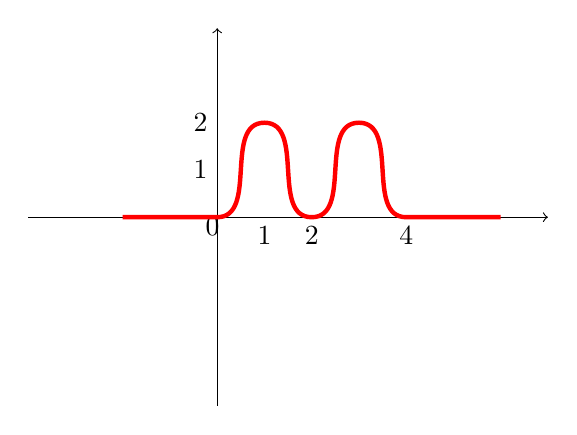
\begin{tikzpicture}[scale=0.60]
\draw[<-] (0,4) -- (0,-4); \draw [<-] (7,0) -- (-4,0);
\draw (0,2) node[left]{$2$}--  (0,1) node[left] {$1$} -- (0,0) --   (-0.,-0.) node[left][below] { }(1,0)
node[below] {$1$} -- (2,0) node[below] {$2$}  -- (4,0) node[below] {$4$};
\node at (-0.1,-0.2) {$0$};
\draw [red,ultra thick] (-2,0) to (0,0) to[out=0,in=180] (1,2)to [out=0,in=180](2,0) to[out=0,in=180] (3,2)
to[out=0,in=180] (4,0) to (6,0);
\end{tikzpicture}



 \section{A piecewise graph} 
 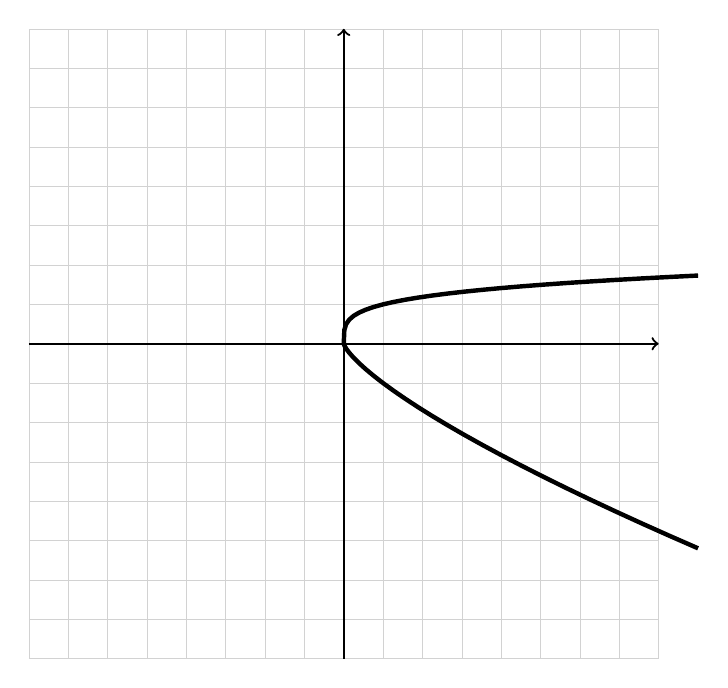
\begin{tikzpicture}
 \begin{scope}[scale=.5]
\draw[help lines, lightgray!70] (-8,-8) grid (8,8);
\draw[thick,->] (-8,0)--(8,0);
	\draw[thick,->] (0,-8)--(0,8);
%\draw [re,very thick] (-4,-4) to (4,4);
\draw[, ultra thick, domain=0:3] plot (\x*\x, {sqrt(\x)});
\draw[, ultra thick, domain=0:3] plot (\x*\x, {-sqrt(\x)*\x});
\end{scope}		
\end{tikzpicture}



 \section{Random graph} 
 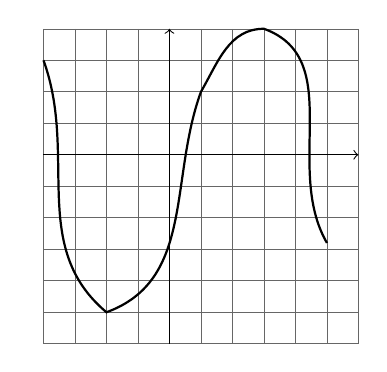
\begin{tikzpicture}
\begin{scope}[scale=.4,rotate=180]
	\draw[help lines, black!60] (-6,-4) grid (4,6);
	\draw[] (-6,0)--(4,0);
	\draw[](0,-4)--(0,6);
	\draw[thick] (-5,2.8)to [out=300,in=160](-3,-4) to [out=0,in=240](-1,-2) to [out=70,in=200](2,5)
	to [out=320,in=110](4,-3);
	\draw[->] (-5.9,0)--(-6,0);
	\draw[->] (0,-3.9)--(0,-4);
\end{scope}
\end{tikzpicture}


 \section{Half-line} 
 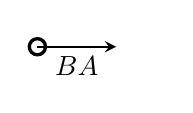
\begin{tikzpicture}	
\begin{scope}[scale=.5]
\draw[->,>=stealth,thick] (-2,0)-- (0,0);
\draw (-1,0)node[below]{$ BA $};
\draw (1,.25)node{};
%\draw[fill] (-0.,0) circle(.21051);
\draw[very thick] (-2,0) circle(.2051);
	\end{scope}		
\end{tikzpicture}


 \section{Ray} 
 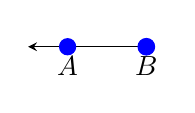
\begin{tikzpicture}	
\begin{scope}[scale=.5]
\draw[<-,>=stealth] (-2,0)-- (1,0);
\draw (-1,0)node[below]{$ A $};
\draw (1,0)node[below]{$ B $};
\draw (1,.25)node{};
\draw[fill,blue] (1,0) circle(.21051);
\draw[fill,blue ] (-1,0) circle(.2051);
	\end{scope}		
\end{tikzpicture}


 \section{A boxed text} 
 \begin{tikzpicture}
\draw (0,0) rectangle (10,2);
\draw (2,1)node[right]{Recueil de Cantiques};	
\end{tikzpicture}


 \section{A graph: touch without crossing} 
 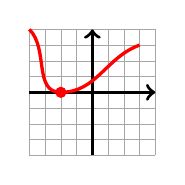
\begin{tikzpicture}
\begin{scope}[scale=.2]
\draw[help lines, gray!70] (-4,-4) grid (4,4);
\draw[very thick,->] (-4,0)--(4,0);
	\draw[very thick,->] (0,-4)--(0,4);
\draw [red,very thick] (-4,4)[out=315,in=180] to (-2,0);
\draw [red,very thick] (-2,0)[out=0,in=200] to (3,3);
%\draw[red, <-,ultra thick, domain=-3:-.12] plot (\x, { -\x*\x +2});
\draw[fill,red] (-2,0) circle (.32);
%\draw[red, ->,ultra thick, domain=.12:4] plot (\x, {4});
%\draw[ red] (0,4) circle (.32);
	\end{scope}		
\end{tikzpicture}


 \section{Alternate interior angles} 
 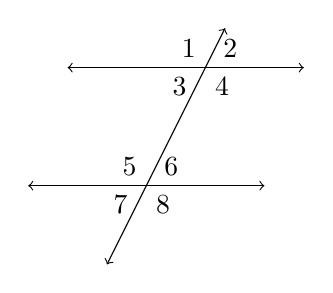
\begin{tikzpicture}	
\begin{scope}[scale=.5]
\draw[<->] (-3,0)-- (3,0);
\draw[<->] (-2,3)-- (4,3);
\draw (1.71,3)node[above right]{2};
\draw (1.5,3)node[above left]{1};
\draw (1.5,3)node[below right]{4};
\draw (1.5,3)node[below left]{3~~};
\draw (0.21,0)node[above right]{6};
\draw (0,0)node[above left]{5};
\draw (0,0)node[below right]{8};
\draw (0,0)node[below left]{7~~};
%\draw (-2,0)node[above right]{$ B$};
%\draw (2,0)node[above right]{$ C $};
%\draw (-1,-2)node[below right]{$D$};
%\draw (1,2)node[right]{$E$};
%\draw[fill] (-0.,0) circle(.21051);
%\draw[fill] (2.,0) circle(.21051);
%\draw[fill] (-2,0) circle(.2051);
%\draw[fill] (-1.,-2) circle(.21051);
%\draw[fill] (1,2) circle(.2051);
%\draw (-1,.25)node{};
\draw[<->] (-1,-2)--(2,4);
	\end{scope}		
\end{tikzpicture}


 \section{Arithmetic sequence} 
 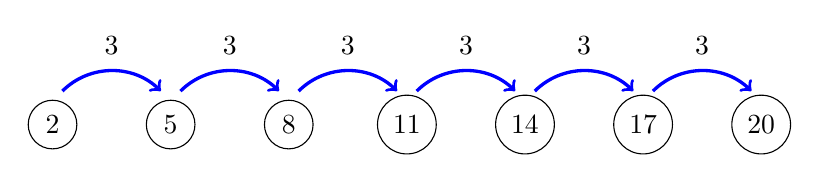
\begin{tikzpicture}[scale=.5]
    \draw(2,0) node[draw,shape=circle]{$2$};
    \foreach \x in { 5, 8, 11, 14, 17, 20}
 {   
 \draw(\x,0) node[draw,shape=circle]{$\x$};
 \draw[->,very thick,blue](\x-2.75,0.85) to[out=45,in=135] (\x-.25,.85);
 \draw (\x-1.5,2) node{$3$};
     
    }
 
    \end{tikzpicture}
    
    
    
 \section{Graph $f(x)=(x-1)^3-2$} 
 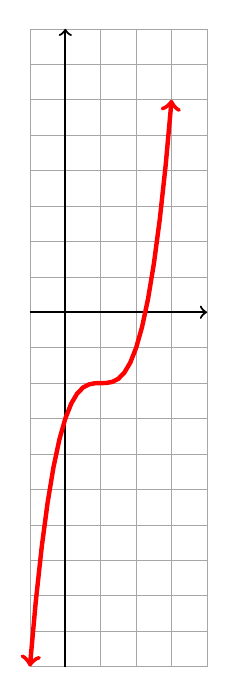
\begin{tikzpicture}
 \begin{scope}[scale=.45]
\draw[help lines, gray!70] (-1,-10) grid (4,8);
\draw[thick,->] (-1,0)--(4,0);
	\draw[thick,->] (0,-10)--(0,8);
%\draw [re,very thick] (-4,-4) to (4,4);
\draw[red, ultra thick, domain=-1:3,<->] plot (\x, {(\x-1)*(\x-1)*(\x-1)-2});
\end{scope}		
\end{tikzpicture}


 \section{Graph: a random one.} 
 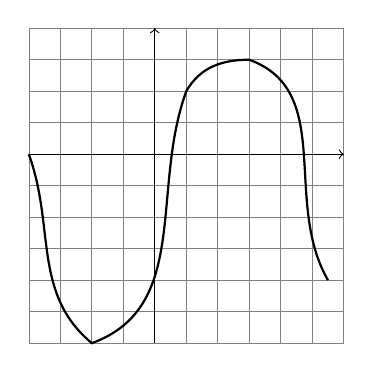
\begin{tikzpicture}
\begin{scope}[scale=.4,rotate=180]
	\draw[help lines, gray] (-6,-4) grid (4,6);
	\draw[] (-6,0)--(4,0);
	\draw[](0,-4)--(0,6);
	\draw[thick] (-5.5,4)to [out=300,in=160](-3,-3) to [out=0,in=240](-1,-2) to [out=70,in=200](2,6)
	to [out=320,in=110](4,0);
	\draw[->] (-5.9,0)--(-6,0);
	\draw[->] (0,-3.9)--(0,-4);
\end{scope}
\end{tikzpicture}


  
 \section{Long underlying (derivative market)} 
 \begin{tikzpicture}
\draw[->]  (-1,0)--(3,0);
\draw[->] (0,-1)--(0,3);
\draw [thick,blue,->] (0,0)--(2.5,2.5)node[right]{$m=1$};
\node [below] at (3,0) {$ S_T $};
\node [right] at (0,3) {Payoff};
%\node [left] at (0,1.5) {$ K $};
\end{tikzpicture}



 \section{x-axis symmetry} 
 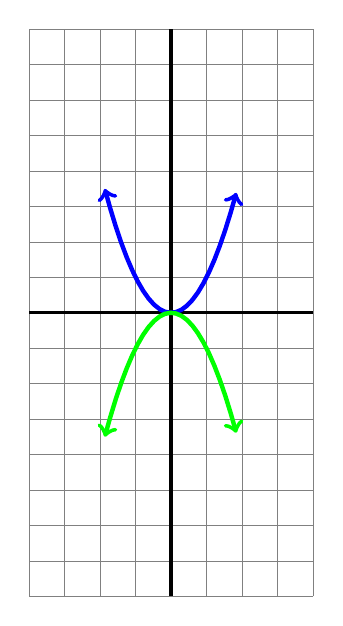
\begin{tikzpicture}	
\begin{scope}[scale=.45]
\draw[help lines] (-4,-8) grid (4,8);
\draw[very thick] (-4,0)--(4,0);
\draw[very thick] (0,-8)--(0,8);
%\draw [red,very thick] (-4,4) to(0,0) to (4,4);
\draw[<->,blue, ultra thick, domain=-1.87:1.84] plot (\x, {(\x*\x)});
\draw[<->,green, ultra thick, domain=-1.87:1.84] plot (\x, {-(\x*\x)});
	\end{scope}		
\end{tikzpicture}


\section{A random graph} 
 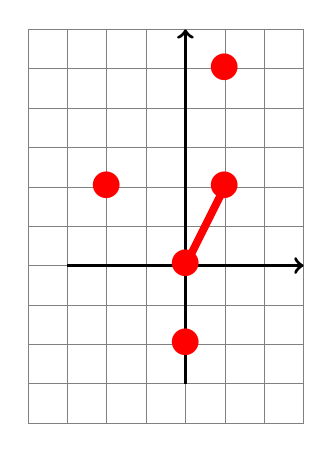
\begin{tikzpicture}	
\begin{scope}[scale=.5]
\draw[help lines] (-4,-4) grid (3,6);
\draw[very thick,->] (-3,0)--(3,0);
	\draw[very thick,->] (0,-3)--(0,6);
\draw [red,thick] (1,2)node{\begin{Huge}$\bullet$\end{Huge}};
\draw [red,thick] (1,5)node{\begin{Huge}$\bullet$\end{Huge}};
\draw [red,thick] (-2,2)node{\begin{Huge}$\bullet$\end{Huge}};
\draw [red,thick] (0,-2)node{\begin{Huge}$\bullet$\end{Huge}};
\draw [red, line width=1mm](0,0)--(1,2);
\draw [red,thick] (0,0)node{\begin{Huge}$\bullet$\end{Huge}};
	\end{scope}		
\end{tikzpicture}


 \section{Floor} 
 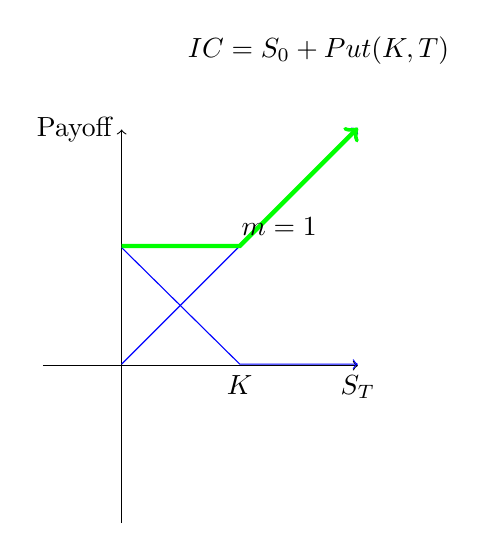
\begin{tikzpicture}
\draw[->]  (-1,0)--(3,0);
\draw[->] (0,-2)--(0,3);
\draw [ blue,->] (0,1.5)--(1.5,0.02)--(3 ,0.02);
\draw [ blue,->] (0,0.02)-- (3 ,3.02);
\draw [ultra thick,green,->] (0,1.52)-- (1.5 ,1.52)--(3,3.02);
\node [below] at (3,0) {$ S_T $};
\node [left] at (0,3) {Payoff};
\node [below] at (1.5,0) {$ K $};
\node[right,below] at (2,2) {$m=1$};
\node at (2.5,4) {$ IC=S_0+Put(K,T) $};
\end{tikzpicture}


 \section{Exterior angle} 
 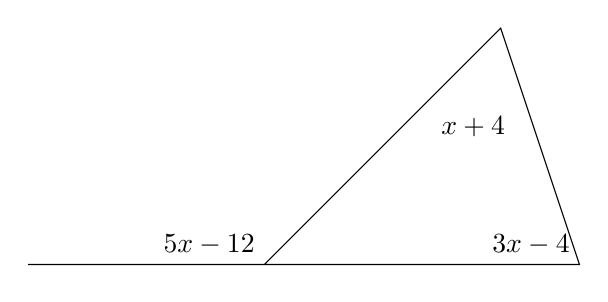
\begin{tikzpicture}
	\draw (-3,0)--(0,0) node[left]{}--(4,0)--(3,3)--(0,0);
\draw (0,0)node[above left]{$ 5x-12 $} ;
\draw (4,0)node[above left]{$ 3x-4 $} ;
\draw (2.65,1.5)node[above]{$ x+4$} ;
\end{tikzpicture}


 \section{Graph $f(x)=\frac1{x^2}$} 
 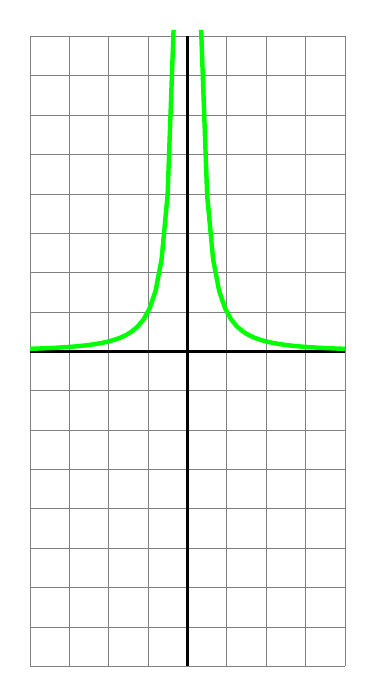
\begin{tikzpicture}	
\begin{scope}[scale=.5]
\draw[help lines] (-4,-8) grid (4,8);
\draw[very thick] (-4,0)--(4,0);
\draw[very thick] (0,-8)--(0,8);
%\draw [red,very thick] (-4,4) to(0,0) to (4,4);
\draw[green, ultra thick, domain=0.35:4] plot (\x, {1/(\x*\x)});
\draw[green, ultra thick, domain=0.35:4] plot (-\x, {1/(\x*\x)});
	\end{scope}		
\end{tikzpicture}


 \section{Gate function} 
 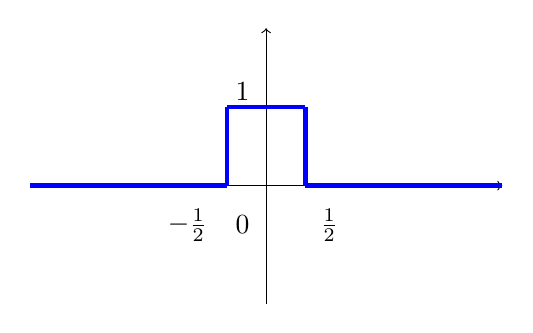
\begin{tikzpicture}[xscale=1,yscale=1]
\draw[<-] (0,2) -- (0,-1.5); \draw [<-] (3,0) -- (-3,0);
\draw [blue, ultra thick,](-3,0) --(-0.5,0);
\draw [blue, ultra thick,](-0.5,1) --(-0.5,0);
\draw [blue, ultra thick,](0.5,1) --(-0.5,1);
\draw [blue, ultra thick,](0.5,1) --(0.5,0);
\draw [blue, ultra thick,](0.5,0) --(3,0);
\node at (-0.3,-0.5) {$0$};
\node at (-1,-0.5) {$-\frac12$};
\node at (0.8,-0.5) {$\frac12$};
\node at (-0.3,1.2) {$1$};
\end{tikzpicture}

 
 \section{Bull spread} 
 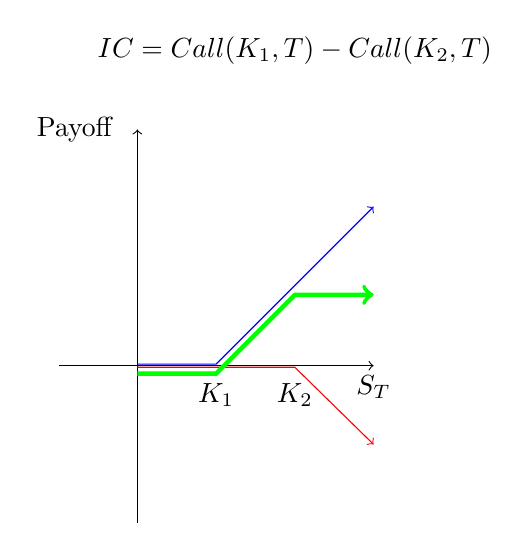
\begin{tikzpicture}
\draw[->]  (-1,0)--(3,0);
\draw[->] (0,-2)--(0,3);
\draw [ blue,->] (0,.02)--(1.,0.02)--(3 ,2.02);
\draw [ red,->] (0,-.02)--(2.,-0.02)--(3 ,-1);
\draw [ultra thick,green,->] (0,-.1)-- (1  ,-.1)--(2,.9)--(3,.9);
\node [below] at (3,0) {$ S_T $};
\node [left] at (-0.2,3) {Payoff};
\node [below] at (1.,-.10) {$ K_1$};
\node [below] at (2.,-.10) {$ K_2$};
%\node[right,below] at (2,2) {$m=1$};
\node at (2,4) {$ IC=Call(K_1,T)-Call(K_2,T) $};
\end{tikzpicture}


 \section{Graph $f(x)=-x^3$} 
 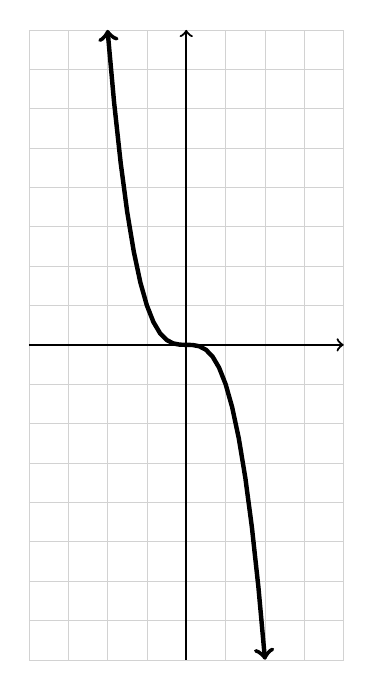
\begin{tikzpicture}
 \begin{scope}[scale=.5]
\draw[help lines, lightgray!70] (-4,-8) grid (4,8);
\draw[thick,->] (-4,0)--(4,0);
	\draw[thick,->] (0,-8)--(0,8);
%\draw [red,very thick] (-4,-4) to (4,4);
\draw[<->, ultra thick, domain=-2:2] plot (\x, {-\x*\x*\x});
\end{scope}		
\end{tikzpicture}


 \section{Graph $f(x)=x^{\frac15}$} 
 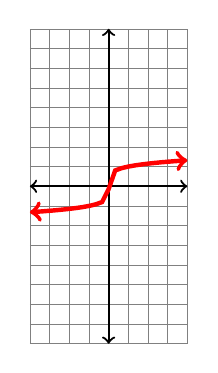
\begin{tikzpicture}	
\begin{scope}[scale=.25]
\draw[help lines] (-4,-8) grid (4,8);
\draw[thick,<->] (-4,0)--(4,0);
\draw[thick,<->] (0,-8)--(0,8);
%\draw [red,very thick] (-4,4) to(0,0) to (4,4);
%\draw[red, ultra thick, domain=.7:4,<->] plot (\x, {1/(\x*\x*\x*\x*\x*\x)});
\draw[red, ultra thick, domain=-4:4,<->] plot ( \x,{\x^(1/5)});
	\end{scope}		
\end{tikzpicture}


 \section{Graph $f(x)=sqrt x$} 
 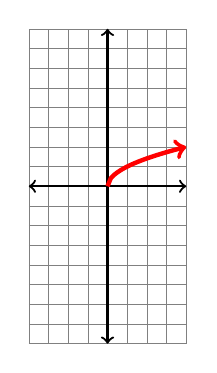
\begin{tikzpicture}	
\begin{scope}[scale=.25]
\draw[help lines] (-4,-8) grid (4,8);
\draw[thick,<->] (-4,0)--(4,0);
\draw[thick,<->] (0,-8)--(0,8);
%\draw [red,very thick] (-4,4) to(0,0) to (4,4);
\draw[red, ultra thick, domain=0:4,->] plot ( \x,{\x^(.5)});
\end{scope}		
\end{tikzpicture}

  
 \section{Cilynder and dome} 
  
 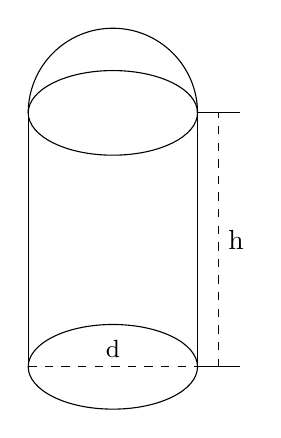
\begin{tikzpicture}
\begin{scope}[scale=1.075]
\draw(0,0) ellipse(1 and .5);
\draw(0,-3) ellipse(1 and .5);
\draw (-1,0) arc(180:0:1);
\draw (-1,-3)--(-1,0);
\draw (1,-3)--(1,0);
\draw[dashed](-1,-3)--(0,-3)node[above]{\small{d}}--(1,-3);
\draw (1,0)--(1.5,0);

\draw (1,-3)--(1.5,-3);
\draw[dashed] (1.25,-3)--(1.25,0);
\draw (1.25, -1.5)node[right]{h};
	
\end{scope}
\end{tikzpicture}


\section{Compactly supported function} 
 
\begin{tikzpicture}[xscale=1,yscale=1]
\draw[<-] (0,2) -- (0,-1); \draw [<-] (3,0) -- (-3,0);
\draw [green, ultra thick,](-2,0) --(-1,0);
\draw [green, ultra thick,](1,0) --(2,0);
\draw[green, ultra thick, domain=-0.98:0.98] plot (\x, {exp(-1/(1-\x*\x))});
\node at (-0.1,-0.2) {$0$};
\node at (-1.1,-0.2) {$-1$};
\node at (1.1,-0.2) {$1$};
\node at (-0.1,1) {$1$};
\end{tikzpicture}


 \section{Sphere} 
 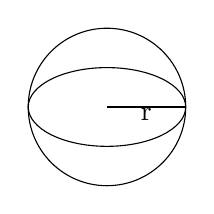
\begin{tikzpicture}
	\draw (0,0) ellipse(1 and .5);
	\draw (0,0)--(1,0);
	\draw (0,0) circle (1);
	\draw (.5,0.1) node[below]{r};
%	\draw (2,0,-.5) node[below right]{w};
%	\draw (1,.5) node[right]{h};
\end{tikzpicture}


 \section{Graph: random} 
 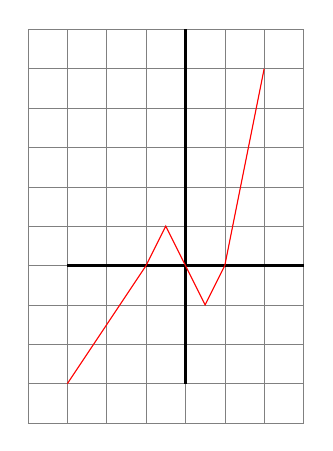
\begin{tikzpicture}	
\begin{scope}[scale=.5]
\draw[help lines] (-4,-4) grid (3,6);
\draw[very thick] (-3,0)--(3,0);
	\draw[very thick] (0,-3)--(0,6);
\draw [red] (-3,-3) to (-1,0) to (-.5,1) to (0,0) 	to (.5 ,-1) to (1,0) to(2,5);
	\end{scope}		
\end{tikzpicture}


 \section{Graph $f(x)=x^2+\frac1{x^2}$} 
 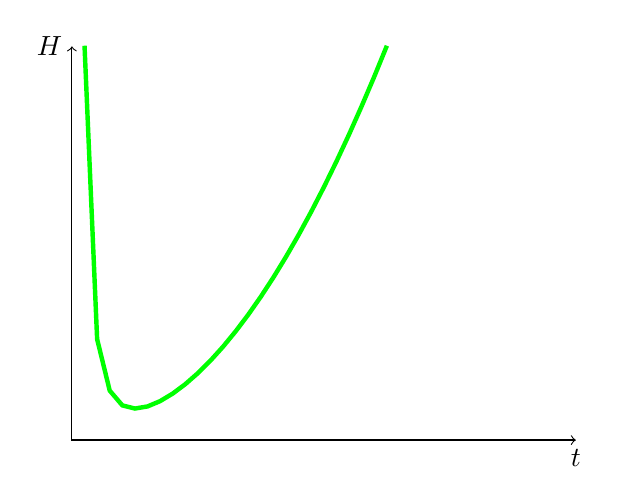
\begin{tikzpicture}[xscale=0.8,yscale=.2]
\draw [<->] (0,25) node[left]{$H$} -- (0,0) -- (8,0) node[below] {$t$};
\draw[green, ultra thick, domain=0.2:5] plot (\x, {1/(\x*\x)+\x*\x});
\end{tikzpicture}


\section{Exponentials: $e^x,2^x,4^4$} 
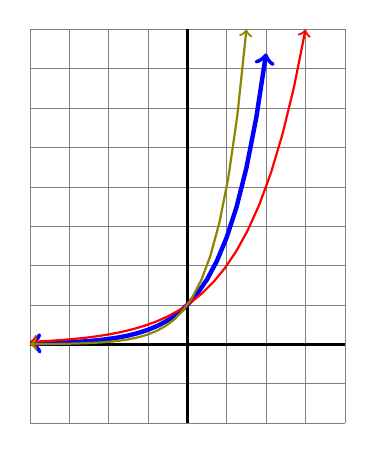
\begin{tikzpicture}	
\begin{scope}[scale=.5]
\draw[help lines] (-4,-2) grid (4,8);
\draw[very thick] (-4,0)--(4,0);
\draw[very thick] (0,-2)--(0,8);
%\draw [red,very thick] (-4,4) to(0,0) to (4,4);
\draw[blue, ultra thick, domain=-4:2,<->] plot (\x, {exp(\x)});
\draw[red, thick, domain=-4:3,<->] plot (\x, {exp(\x*ln(2))});
\draw[olive, thick, domain=-4:1.50,<->] plot (\x, {exp(\x*ln(4))});
%\draw[green, ultra thick, domain=0.35:4] plot (-\x, {1/(\x*\x)});
\end{scope}		
\end{tikzpicture}



 \section{Two graphs} 
 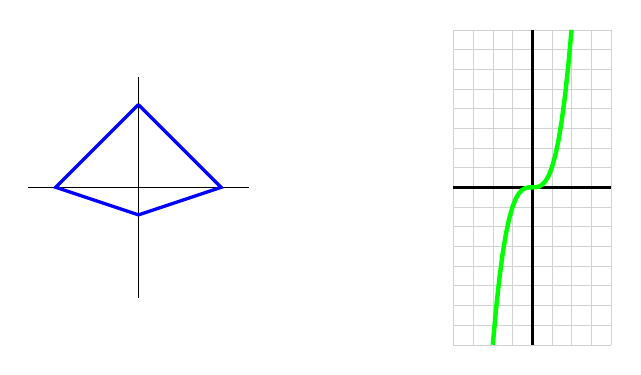
\begin{tikzpicture}
 \begin{scope}[scale=.35]
\draw (-4,0)--(4,0);
	\draw (0,-4)--(0,4);
	\draw[blue,very thick] (0,3)--(-3,0)--(0,-1)--(3,0)--(0,3);
	\end{scope}
	
\begin{scope}[xshift=5cm ,scale=.5]
\begin{scope}[scale=.5]
\draw[help lines, lightgray!70] (-4,-8) grid (4,8);
\draw[very thick] (-4,0)--(4,0);
	\draw[very thick] (0,-8)--(0,8);
%\draw [red,very thick] (-4,-4) to (4,4);
\draw[green, ultra thick, domain=-2:2] plot (\x, {\x*\x*\x});
	\end{scope}	
	\end{scope}		
\end{tikzpicture}


 \section{Piecewise function} 
 \begin{tikzpicture}
 \begin{scope}[scale=1]
\draw[help lines, gray] (-4,-4) grid (4,4);
\draw[thick,->] (-4,0)--(4,0);
	\draw[thick,->] (0,-4)--(0,4);
%\draw [re,very thick] (-4,-4) to (4,4);
\draw[<-, ultra thick, domain=-3:-.1] plot (\x, {2});
\draw[fill] (0,2) circle (.2);
\draw[ ultra thick, domain=.1:1] plot (\x, \x*\x);
\draw (0,0) circle (.2);
\draw[->, ultra thick, domain=1:2] plot (\x*\x, {\x});
\end{scope}		
\end{tikzpicture}


 \section{Graph $ f(x)=x^5$} 
 \begin{tikzpicture}	
\begin{scope}[scale=.25]
\draw[help lines] (-4,-8) grid (4,8);
\draw[thick,<->] (-4,0)--(4,0);
\draw[thick,<->] (0,-8)--(0,8);
%\draw [red,very thick] (-4,4) to(0,0) to (4,4);
\draw[red, ultra thick, domain=-1.5:1.5,<->] plot (\x, {\x*\x*\x*\x*\x});

	\end{scope}	
	
\end{tikzpicture}


 \section{A rectangle} 
 
 \begin{tikzpicture}	
\begin{scope}[scale=.5]
\draw (0,0) rectangle (4,3);
	\end{scope}		
\end{tikzpicture}


 \section{Line} 
 \begin{tikzpicture}	
\begin{scope}[scale=.5]
\draw[<->,>=stealth,thick] (-2,0)-- (2,0);
\draw (-1,0)node[below]{$ A $};
\draw (1,0)node[below]{$ B $};
\draw (1,.25)node{};
\draw[fill,blue ] (-1,0) circle(.051);
\draw[fill,blue ] (1,0) circle(.051);
	\end{scope}		
\end{tikzpicture}


 \section{Identity function} 
 \begin{tikzpicture}	
\begin{scope}[scale=.5]
\draw[help lines] (-4,-4) grid (4,4);
\draw[very thick] (-4,0)--(4,0);
	\draw[very thick] (0,-4)--(0,4);
\draw [red,very thick] (-4,-4) to (4,4);
	\end{scope}		
\end{tikzpicture}


 

 \section{Graph $f(x)=x^3$} 
 \begin{tikzpicture}
\begin{scope}[scale=.25]
\draw[help lines, gray!70] (-4,-8) grid (4,8);
\draw[very thick,->] (-4,0)--(4,0);
	\draw[very thick,->] (0,-8)--(0,8);
%\draw [red,very thick] (-4,-4) to (4,4);
\draw[blue,<->, ultra thick, domain=-2:2] plot (\x, {\x*\x*\x});
	\end{scope}		
\end{tikzpicture}


\section{Balls and gradian} 
\begin{tikzpicture}
\foreach \x in {1,2,...,10}
\shade[ball color=red!\x 0!green] (\x,0) circle (3mm);
\end{tikzpicture}


 \section{Graph $f(x)=0.2x^2$} 
 \begin{tikzpicture}
\begin{scope}[scale=.2]
\draw[help lines, gray!70] (-4,-4) grid (4,4);
\draw[very thick,->] (-4,0)--(4,0);
	\draw[very thick,->] (0,-4)--(0,4);
%\draw [red,very thick] (-4,4)[out=315,in=180] to (-2,0);
%\draw [red,very thick] (-2,0)[out=0,in=200] to (3,3);
%\draw[red, <-,ultra thick, domain=-3:-.12] plot (\x, { -\x*\x +2});
%\draw[fill,red] (-2,0) circle (.32);
\draw[red, <->,ultra thick, domain=-4:4] plot (\x, {0.2*\x*\x});
%\draw[ red] (0,4) circle (.32);
	\end{scope}		
\end{tikzpicture}


 \section{Triangulation} 
 \begin{tikzpicture}[scale=4.5]
\draw (0,0)node[below]{$p(1)$}--(1,0)node[below]{$p(3)$}--(1,1)node[above]{$p(9)$}--(0,1)node[above]{$p(7)$}--(0,0)--(1,1)--(.5,1);
\draw (0,.5)node[left]{$p(4)$}--(.5,1)node[above right]{$p(8)$};
\draw (0,.5)--(1,.5)node[right]{$p(6)$};
\draw (0.5,0)node[below]{$p(2)$}--(.5,1);
\draw (0.5,0)--(1,.5);
\node at (.4,.55){\scalebox{.8}{$p(5)$}};
\node at (.35,.125){$t(1)$};
\node at (.15,.315){$t(2)$};
\node at (.35,.725){$t(5)$};
\node at (.15,.825){$t(6)$};
\node at (.85,.125){$t(3)$};
\node at (.65,.325){$t(4)$};
\node at (.85,.625){$t(7)$};
\node at (.65,.825){$t(8)$};
%\draw (.25,.425)node[circle,draw]{\scalebox{.4}{$t(2)$}};
\end{tikzpicture}



 \section{Perpendicular to a line} 
 \begin{tikzpicture}[scale=.6]
 \begin{scope}[rotate=0]
  \draw[very thick] (-3,-3.464)node[below right]{$B$}--
(3,-3.464)node[below left]{$C$};
\draw (-140:4cm)node[left]{$ $} arc (-140:-40:4cm);
% \draw (--120:4cm)node[left]{$A$} arc (-120:40:4cm);
% \draw (--140:4cm)node[left]{$A$} arc (-140:40:4cm);
\draw[very thick] (0,3)--(0,-8);
 \draw (0.5,0.7) node{$A$};
% \draw(4.1 ,2.5) node[right]{$(C)$};
\begin{scope}[shift=(-120:4cm),xscale=1]
\draw (-100:4cm) arc (-100:100:4cm);
%\draw(4.1 ,2.5) node[right]{$(C')$};
\end{scope}
\begin{scope}[shift=(-60:4cm),xscale=-1]
\draw (-100:4cm) arc (-100:100:4cm);
%\draw(4.1 ,2.5) node[right]{$(C')$};
\end{scope}
 \end{scope}
\end{tikzpicture}

 \section{Crossing Lines} 
 \begin{tikzpicture}
	\begin{scope}[scale=1]
\draw [help lines] (-3,-3) grid (3,3);
\draw[->,thick] (-3,0)--(3,0);
\draw[->,thick] (0,-3,0)--(0,3,0);
\draw[<->,blue,thick] (-3,-2)--(3,3);	
\draw[<->,red,thick] (-3,3)--(3,1);
\end{scope}	
\end{tikzpicture}


 \section{Affine piecewise function} 
 \begin{tikzpicture}	
\begin{scope}[scale=.83]
\draw[help lines] (-3,-3) grid (3,3);
\draw [very thick](-3,0)--(3,0);
	\draw [very thick](0,-3)--(0,3);
\draw [<->,red,thick]  (-1.5,-1.85)--(-1,0)
--(-.5,.375)--(.0,0)--(.5,-.375)--(1,0)--(1.5,1.875);
	\end{scope}		
\end{tikzpicture}


 \section{A filled triangle} 
 \begin{tikzpicture}
\draw [help lines] (-2,-2) grid (2,2 );
\draw[fill=gray!50](-1,-.167)--(1,.5)--(-1,.5)--(-1,-.167);
\node at (1.8,0.2){t};	
\node at (-.2,1.8){s};
\draw[->](0,0)--(0,1)node[above left]{$  j $}; 
\draw[->](0,0)--(1,0)node[below left]{$  i $};
\end{tikzpicture}


 \section{Put-Call Parity} 
 \begin{tikzpicture}
\draw[->]  (-1,0)--(3,0);
\draw[->] (0,-2)--(0,3);
\draw [ blue,->] (0,.02)--(1.5,0.02)--(3 ,1.5);
\draw [ red,->] (0,-1.502)--(1.5,0.02)--(3 ,.02);
\draw [ultra thick,green,->] (0,-1.4)-- (1.5 ,.1)--(3,1.6);
\node [below] at (3,0) {$ S_T $};
\node [left] at (-0.2,3) {Payoff};
\node [below] at (1.5,0) {$ K $};
\node[right,below] at (2,2) {$m=1$};
\node at (2.3,4) {$ IC=Call(K,T)-Put(K,T) $};
\end{tikzpicture}


 \section{Horizontal translation} 
 \begin{tikzpicture}	
\begin{scope}[scale=.5]
\draw[help lines] (-4,-8) grid (4,8);
\draw[very thick] (-4,0)--(4,0);
\draw[very thick] (0,-8)--(0,8);
%\draw [red,very thick] (-4,4) to(0,0) to (4,4);
\draw[<->,blue, ultra thick, domain=-1.87:1.84] plot (\x, {(\x*\x)});
\draw[<->,green, ultra thick, domain=-1.87:1.84] plot (\x+1, {(\x*\x)});
\draw[<->,red, ultra thick, domain=-1.87:1.84] plot (\x-2, {(\x*\x)});
	\end{scope}		
\end{tikzpicture}


 \section{Put} 
 \begin{tikzpicture}
\draw[->]  (-1,0)--(3,0);
\draw[->] (0,-1)--(0,3);
\draw [thick,blue,->] (0,1.5)--(1.5,0)--(2.5,0);
\node [below] at (3,0) {$ S_T $};
\node [left] at (0,3) {Payoff};
\node [below] at (1.5,0) {$ K $};
\node[right,below] at (2,2) {$m=-1$};
\node at (2.5,3) {$ IC=Put(K,T) $};
\end{tikzpicture}


 \section{A line} 
 \begin{tikzpicture}	
\begin{scope}[scale=.345]
\draw[help lines] (-4,-4) grid (3,6);
\draw[very thick] (-3,0)--(3,0);
	\draw[very thick] (0,-3)--(0,6);
\draw [red,very thick,<->] (-3,-3) to (-1,0)  to (2,5);
	\end{scope}		
\end{tikzpicture}


 \section{Butterfly Spread} 
 
 \begin{tikzpicture}
\draw[->,gray]  (-1,0)--(5,0);
\draw[->,gray] (0,-3)--(0,2);
\draw [ blue,->] (0,1)--(1.,-0.02)--(4.5 ,-.02);
\draw [ blue,->] (0,-2)--(2.,-0.02)--(4.5 ,-.02);
\draw [ red,->] (0,.02)--(2.,0.02)--(5 ,-3);
\draw [ red,->] (0,.02)--(4.,0.02)--(5 ,1);
\draw [ultra thick,green,->] (0,-1.1)-- (1  ,-1.1)--(2,-.1)--(4,-2.1)--(5,-2.1);
\node [below] at (5,0) {$ S_T $};
\node [left] at (-0.2,2) {Payoff};
\node [below] at (1.,-.10) {$ K_1$};
\node [below] at (2.,-.10) {$ K_2$};
\node [below] at (4.,-.10) {$ K_3$};
%\node[right,below] at (2,2) {$m=1$};
\node at (2,3) {$ IC=Call(K3,T)-Call(K2,T)+Put(K1,T)-Put(K2,T) $};
\end{tikzpicture}


 \section{Ratio spread} 
 \begin{tikzpicture}
\draw[->,gray]  (-1,0)--(5,0);
\draw[->,gray] (0,-3)--(0,4);
\draw [ blue,->] (0,0)--(1 ,0)--(3,4);
\draw [red,->] (0,0)--(2  ,0)--(3,-4);
\draw [ultra thick,green,->] (0,0)--(1,0)--(2,1)--(3,-1)--(4,-3);
\node [below] at (5,0) {$ S_T $};
\node [left] at (-0.2,2) {Payoff};
\node [below] at (1.,-.10) {$ K_1$};
\node [below] at (2.,-.10) {$ K_2$};
%\node [below] at (4.,-.10) {$ K_3$};
%\node[right,below] at (2,2) {$m=1$};
\node at (2,5) {$ IC=2Call(K1,T)-4Call(K2,T) $};
\end{tikzpicture}


 \section{Gradient and balls} 
 \begin{tikzpicture}
 \foreach \x in {0,1,...,11}
\shade[ball color=yellow!\x 0!red] (\x,0) circle (3mm);
\end{tikzpicture}



 \section{CLosed curve} 
 \begin{tikzpicture}	
\begin{scope}[scale=.5]
\draw (0,0) to [in=200,out=0](2,3) to [out=20,in=90] (4,1) to [out=300,in=360] (0,0);
	\end{scope}		
\end{tikzpicture}


 \section{Points in a plane} 
 \begin{tikzpicture}	
\begin{scope}[scale=1]
%\draw[help lines] (-4,-8) grid (4,8);
%\draw[very thick] (-4,0)--(4,0);
%\draw[very thick] (0,-8)--(0,8);
%\draw [red,very thick] (-4,4) to(0,0) to (4,4);
%\draw[green, ultra thick, domain=0.35:4] plot (\x, {1/(\x*\x)});
%\draw[green, ultra thick, domain=0.35:4] plot (-\x, {1/(\x*\x)});
\draw  (0,0)--(4,0)--(5,4)--(1,4)--(0,0);
%\draw[<->,>=stealth] (0.5,0.5)-- (3.4,3.4);
\draw (1.2,1.2)node[right]{$ A $};
\draw (2.6,2.6)node[right]{$ B $};
\draw (3,2)node[right]{$ C $};
\draw[fill,blue ] (1.2,1.2) circle(.051);
\draw[fill,blue ] (2.6,2.6) circle(.051);
\draw[fill,blue ] (3,2) circle(.051);
	\end{scope}		
\end{tikzpicture}

\section{Crossing lines} 
\begin{tikzpicture}	
\begin{scope}[scale=.5]
\draw[<->] (-3,0)-- (3,0);
\draw (0,0)node[above right]{$ A $};
\draw (-2,0)node[above right]{$ B$};
\draw (2,0)node[above right]{$ C $};
\draw (-1,-2)node[below right]{$D$};
\draw (1,2)node[right]{$E$};
\draw[fill] (-0.,0) circle(.21051);
\draw[fill] (2.,0) circle(.21051);
\draw[fill] (-2,0) circle(.2051);
\draw[fill] (-1.,-2) circle(.21051);
\draw[fill] (1,2) circle(.2051);
\draw (-1,.25)node{};
\draw (-2,-4)--(2,4);
	\end{scope}		
\end{tikzpicture}


 \section{A triangle} 
 \begin{tikzpicture}
 \begin{scope}[scale=.5]
\draw[help lines, gray!70] (-4,-8) grid (4,8);
\draw[thick,->] (-4,0)--(4,0);
	\draw[thick,->] (0,-8)--(0,8);
%\draw [re,very thick] (-4,-4) to (4,4);
\draw[, ultra thick] (-2,-3)--(3,5)--(2,-2)--(-2,-3);
\end{scope}		
\end{tikzpicture}


 \section{Long Bond} 
 \begin{tikzpicture}
\draw[->]  (-1,0)--(3,0);
\draw[->] (0,-1)--(0,3);
\draw [thick,blue,->] (0,1.5)--(2.5,1.5);	
\node [below] at (3,0) {$ S_T $};
\node [left] at (0,3) {Payoff};
\node [right] at (0,3) {$ IC=K\nu^T $ };
\node [left] at (0,1.5) {$ K $};
\end{tikzpicture}




\section{Graph $f(x)=x^{2/3}$} 
 \begin{tikzpicture}
 \begin{scope}[scale=.5]
\draw[help lines, lightgray!70] (-8,-8) grid (8,8);
\draw[thick,->] (-8,0)--(8,0);
	\draw[thick,->] (0,-8)--(0,8);
%\draw [re,very thick] (-4,-4) to (4,4);
\draw[, ultra thick, domain=-2:2] plot (\x*\x*\x, {\x*\x});
\end{scope}		
\end{tikzpicture}


 \section{Graph $x=y^{2/3}$} 
 \begin{tikzpicture}
 \begin{scope}[scale=.5]
\draw[help lines, lightgray!70] (-4,-8) grid (4,8);
\draw[thick,->] (-4,0)--(4,0);
	\draw[thick,->] (0,-8)--(0,8);
%\draw [re,very thick] (-4,-4) to (4,4);
\draw[, ultra thick, domain=-2:2] plot (\x*\x, {-\x*\x*\x});
\end{scope}		
\end{tikzpicture}

  \section{Crossing x-axis} 
 \begin{tikzpicture}
\begin{scope}[scale=.2]
\draw[help lines, gray!70] (-4,-4) grid (4,4);
\draw[very thick,->] (-4,0)--(4,0);
	\draw[very thick,->] (0,-4)--(0,4);
\draw [red,very thick] (-4,-4)[out=45,in=200] to (-1,2);
\draw [red,very thick] (-1,2)[out=20,in=200] to (3,-3);
%\draw[red, <-,ultra thick, domain=-3:-.12] plot (\x, { -\x*\x +2});
\draw[fill,red] (1,0) circle (.32);
%\draw[red, ->,ultra thick, domain=.12:4] plot (\x, {4});
%\draw[ red] (0,4) circle (.32);
	\end{scope}		
\end{tikzpicture}


 \section{Two graphs} 
 \begin{tikzpicture}
 \begin{scope}[scale=.5]
\draw (-3,0)--(3,0);
	\draw (0,-3)--(0,3);
	\draw[blue] (0,0)circle[radius=2];
	\end{scope}
	
\begin{scope}[xshift=5cm ,scale=.5]
\draw (-3,0)--(3,0);
	\draw (0,-3)--(0,3);
	\draw [red] (-3,1) to [out=40,in=180] (-1,-1) to [out=70,in=180] (1,1)
to [out=0,in=180] (2.5,0) to [out=0,in=-135] (3,1) ;
	\end{scope}		
\end{tikzpicture}


 \section{Graph $ f(x)=\frac{1}{x^5}$} 
 \begin{tikzpicture}	
\begin{scope}[scale=.25]
\draw[help lines] (-4,-8) grid (4,8);
\draw[thick,<->] (-4,0)--(4,0);
\draw[thick,<->] (0,-8)--(0,8);
%\draw [red,very thick] (-4,4) to(0,0) to (4,4);
\draw[red, ultra thick, domain=.65:4,<->] plot (\x, {1/(\x*\x*\x*\x*\x)});
\draw[red, ultra thick, domain=-4:-.65,<->] plot (\x, {1/(\x*\x*\x*\x*\x)});
	\end{scope}	
	
\end{tikzpicture}


 \section{Triangulation} 
 \begin{tikzpicture}
\draw[help lines] (-1,-1) grid (3,4);
\draw (0,0)--(0,3)--(2,3)--(2,0)--(0,0);
\draw (0,1)--(2,1);\draw (0,2)--(2,2);%
\draw (2,0)--(0,2);
\draw (2,1)--(0,3);
\draw (1,0)--(0,1);
\draw (2,2)--(1,3);
%\draw (0,2)--(3,2);%draw (0,3)--(4,3);
\filldraw[black] (1,1) circle (2pt);
\filldraw[black] (1,2) circle (2pt);
%\draw (0,0)--(4,0)--(2,2)--(0,2)--(0,0);
% \draw (0,2)--(2,0);
% % \filldraw[black] (0,0) circle (2pt) node[anchor=south] {Intersection point};
\draw [ pattern color = black!30,pattern = north east lines ]
(1,1)--(0,2)--(1,2)--(2,1)--(1,1) ;
\draw  (-1,0)  node[left] { $(j-1)h$};
\draw  (-1,1)  node[left] { $jh$};
\draw  (-1,2)  node[left] { $\bar jh$};
\draw  (-1,3)  node[left] { $(\bar j+1)h$};
\draw  (-.5,-1)  node[left,below] { $(i-1)h$};
\draw  (1,-1)  node[below] { $ih=\bar ih$};
\draw  (2.5,-1)  node[right,below] { $( i+1)h$};
\draw  (.65,1.75)  node { $T_1$};
\draw  (1.25,1.25)  node { $T_2$};
% \draw  (3.5,0)  node[rigth, below] {$v$ at $((i+1)h,jh)$};
% \draw  (-1,2)  node[left, above] {$w$ at $(ih,(j+1)h)$};
% \draw  (3.5,2)  node[rigth, above] {$t$ at $((i+1)h,(j+1)h)$};
% \draw (.5,.5) node[above,rigth] {$T^1_{ij}$};
% \draw (1.5,.6) node[above,rigth] {$T^2_{ij}$};
\end{tikzpicture}


 \section{Trapezoid} 
 \begin{tikzpicture}
	\draw(0,0)--(4,0)--(2,2)--(0.5,2)--(0,0);
	\draw (1,0)node[below]  {4cm};
	\draw (1,2)node[above]  {1.5cm};
	\draw (.5,0)--(.5,2);
	\draw  (0.5,1)node[right]{2cm};
	%\draw (2,1)node[right] {2cm};
\end{tikzpicture}


 \section{Curve} 
 \begin{tikzpicture}	
\begin{scope}[scale=.5]
\draw (0,0) to [in=200,out=0](2,3);
\draw (0,2) to [out=20,in=90] (4,1) to [out=300,in=360] (0,-1);
	\end{scope}		
\end{tikzpicture}


 \section{Triangles} 
 \begin{tikzpicture}
 \draw (0,0)--(2,0)--(2,2)--(0,2)--(0,0);
 \draw (0,2)--(2,0);
% \filldraw[black] (0,0) circle (2pt) node[anchor=south] {Intersection point};
\draw  (-1,0)  node[left, below] {$u$ at $(ih,jh)$};
\draw  (3.5,0)  node[right, below] {$v$ at $((i+1)h,jh)$};
\draw  (-1,2)  node[left, above] {$w$ at $(ih,(j+1)h)$};
\draw  (3.5,2)  node[right, above] {$t$ at $((i+1)h,(j+1)h)$};
\draw (.5,.5) node[above,right] {$T^1_{ij}$};
\draw (1.5,.6) node[above,right]{$T^2_{ij}$};
\end{tikzpicture}


 \section{Segment} 
 \begin{tikzpicture}	
\begin{scope}[scale=1]
%\draw[help lines] (-4,-8) grid (4,8);
%\draw[very thick] (-4,0)--(4,0);
%\draw[very thick] (0,-8)--(0,8);
%\draw [red,very thick] (-4,4) to(0,0) to (4,4);
%\draw[green, ultra thick, domain=0.35:4] plot (\x, {1/(\x*\x)});
%\draw[green, ultra thick, domain=0.35:4] plot (-\x, {1/(\x*\x)});
\draw  (0,0)rectangle (4,4);
\draw[<->,>=stealth] (0.5,0.5)-- (3.4,3.4);
\draw (1.2,1.2)node[right]{$ A $};
\draw (2.6,2.6)node[right]{$ B $};
\draw (3,2)node[right]{$ l $};
\draw[fill,blue ] (1.2,1.2) circle(.051);
\draw[fill,blue ] (2.6,2.6) circle(.051);
	\end{scope}		
\end{tikzpicture}


\section{A polygon} 
 \begin{tikzpicture}	
\begin{scope}[scale=.5]
\draw (0,0)--(3,0)--(0,3)--(1,1.5)--(0,0);
	\end{scope}		
\end{tikzpicture}


 \section{Reverse Cap} 
 \begin{tikzpicture}
\draw[->]  (-1,0)--(3,0);
\draw[->] (0,-2)--(0,3);
\draw [ blue,->] (0,-.02)--(1.5,-0.02)--(3 ,-1.5);
\draw [ blue,->] (0,-0.02)-- (3 ,2.98);
\draw [ultra thick,green,->] (0,0)-- (1.5 ,1.5)--(3,1.5);
\node [below] at (3,0) {$ S_T $};
\node [left] at (0,3) {Payoff};
\node [below] at (1.5,0) {$ K $};
\node[right,below] at (2,2) {$m=1$};
\node at (2.5,3) {$ IC=S_0-Call(K,T) $};
\end{tikzpicture}


 
 \section{Reflexion about y-axis} 
 \begin{tikzpicture}	
\begin{scope}[scale=.5]
\draw[help lines] (-4,-8) grid (4,8);
\draw[very thick] (-4,0)--(4,0);
\draw[very thick] (0,-8)--(0,8);
%\draw [red,very thick] (-4,4) to(0,0) to (4,4);
\draw[<->,blue, ultra thick, domain=-1.87:1.84] plot (\x, {(\x*\x*\x)+1});
\draw[<->,green, ultra thick, domain=-1.87:1.84] plot (-\x, {(\x*\x*\x)+1});
%\draw[<->,red, ultra thick, domain=-1.87:1.84] plot (\x-2, {(\x*\x)});
	\end{scope}		
\end{tikzpicture}


 \section{Dilation y-axis} 
 \begin{tikzpicture}	
\begin{scope}[scale=.5]
\draw[help lines] (-4,-2) grid (4,8);
\draw[very thick] (-4,0)--(4,0);
\draw[very thick] (0,-2)--(0,8);
%\draw [red,very thick] (-4,4) to(0,0) to (4,4);
\draw[<->,blue, ultra thick, domain=-1.87:1.84] plot (\x, {(\x*\x)+1});
\draw[<->,green, ultra thick, domain=-1.87:1.84] plot (\x, {2*(\x*\x)+2});
\draw[<->,red, ultra thick, domain=-1.87:1.84] plot (\x, {.5*(\x*\x)+.5});
	\end{scope}		
\end{tikzpicture}


 \section{Translation y-axis} 
 \begin{tikzpicture}	
\begin{scope}[scale=.45]
\draw[help lines] (-4,-8) grid (4,8);
\draw[very thick] (-4,0)--(4,0);
\draw[very thick] (0,-8)--(0,8);
%\draw [red,very thick] (-4,4) to(0,0) to (4,4);
\draw[<->,blue, ultra thick, domain=-1.87:1.84] plot (\x, {(\x*\x*\x)});
\draw[<->,green, ultra thick, domain=-1.87:1.84] plot (\x, {1+(\x*\x*\x)});
\draw[<->,red, ultra thick, domain=-1.87:1.84] plot (\x, {-.5+(\x*\x*\x)});
	\end{scope}		
\end{tikzpicture}


 \section{Long Forward} 
 \begin{tikzpicture}
\draw[->]  (-1,0)--(3,0);
\draw[->] (0,-2)--(0,3);
\draw [thick,blue,->] (0,-1.5)--(1.5,0)--(3.5,2);
\node [below] at (3,0) {$ S_T $};
\node [left] at (0,3) {Payoff};
\node [below] at (1.5,0) {$ K $};
\node[right,below] at (2,2) {$m=1$};
\node at (2.5,3) {$ IC=0 $};
\end{tikzpicture}
 
 


 \section{Graph exponential} 
 \begin{tikzpicture}	
\begin{scope}[scale=.25]
\draw[help lines] (-4,-2) grid (4,8);
\draw[very thick] (-4,0)--(4,0);
\draw[very thick] (0,-2)--(0,8);
%\draw [red,very thick] (-4,4) to(0,0) to (4,4);
\draw[blue, ultra thick, domain=-4:2] plot (\x, {exp(\x)});
%\draw[green, ultra thick, domain=0.35:4] plot (-\x, {1/(\x*\x)});
	\end{scope}		
\end{tikzpicture}


 \section{triangle, rectangle and half-disk} 
 \begin{tikzpicture}
\draw(0,0)--(4,0);
\draw(4,0) arc(-90:90:1)--(1,2)--(0,0);
\draw[dashed] (1,2.3)--(4,2.3);
\draw (2.75,2.3) node[above]{a};
\draw[dashed] (1,0)--(1,2);
\draw (1,1) node[right]{b};
\draw[dashed] (0,-.3)--(4,-.3);
\draw (2,-.3) node[below]{c};
\end{tikzpicture}


 \section{Circunscribe circle} 
 \begin{tikzpicture}
\draw (0,0)node[below]{$B$}--
(7,0)node[below]{$C$}--
(3,5)node[above]{$A$};
\draw (0:1cm) arc (0:59:1cm);
\draw (42:1cm)node{$=$};
\draw (14:1cm)node{$=$};
\begin{scope}[xshift=7cm,xscale=-1]
 \draw (42:1.5cm)node{$-$};
\draw (12.5:1.5cm)node{$-$};
\draw (0:1.5cm) arc (0:51:1.5cm);
\end{scope}
%\draw (0:1.2cm) arc (0:20:1.2cm);
\draw (3,5)--(0,0);
\draw (3.214, 1.82)--
(0, 0);
\draw (3.214, 1.82)--
(7, 0);
\node[above] at (3.214, 1.82){$I$};
%\draw --(3, 5);
\draw (3.214, 1.82)--
(1.654, 2.756)node[above left]{$E$};
\draw (3.214, 1.82)--
(4.635, 2.957)node[above right]{$G$};
\draw (3.214, 1.82)--
(3.214, 0)node[below]{$F$};
\rect{3.214}{0}{0.35}{0}
\rect{4.635}{2.957}{-.25}{-.2}
\rect{1.654}{2.756}{.25}{-.15}
\end{tikzpicture}


 \section{Geometric contruction} 
 \begin{tikzpicture}
%\draw[help lines](-3,-2)grid(8,5);
%   \coordinate (A) at (-6,0);
% \coordinate (B) at (6,3);
% \coordinate (C) at (0,1.5);
\draw (0,0)node[below]{$B$}--++(7,0)node[below]{$C$}
--++(-3,4)node[above]{$A$}--(0,0);
\draw (2.5,2.5)node(M)[left]{$M$}--++(2.625,0)node(M1)[right]{$M'$};
\draw (2.5,2.5)--(2.5,0)node[below]{$H$};
\draw (2.5,2.5)++(2.625,0)--(5.125,0)node[below]{$H'$};
\rect {2.5} {0} {0.2} 0
\rect {5.125} {0} {0.2} 0
\draw (2.5,2.5)--(4.18, 3.76)node[right]{$P$};
\draw (5.125,2.5)--(3.81,3.81)node[left]{$P'$};
%(4.4799999999999995, 3.3599999999999994)
\end{tikzpicture}





\section{Constant} 
 \begin{tikzpicture}	
\begin{scope}[scale=.5]
\draw[help lines] (-4,-4) grid (4,4);
\draw[very thick] (-4,0)--(4,0);
	\draw[very thick] (0,-4)--(0,4);
\draw [red,very thick] (-4,2) to (4,2);
	\end{scope}		
\end{tikzpicture}


 \section{Curve, neighborhood} 
 \begin{tikzpicture}
\begin{scope}
\coordinate (p) at (0,0);
\coordinate (q) at (2,1);
\coordinate (w) at (2.5,1.5);
\coordinate (C) at (.5,.5);
\coordinate (D) at (1,.75);
\coordinate (E) at (3,1.5);
\draw[style=dashed] (2,1) circle (1); 
\node[left] at (p) {$p$};
\node[right] at (q) {$q$}; 
\node[left] at (w) {$w$};
\draw[line width=2pt] (0, 0) .. controls(.5,.5) .. (2, 1);
\draw [line width=2pt] (q) .. controls(2.75,1.75) .. (w);
\end{scope}
\end{tikzpicture}


 \section{Cylinder} 
 \begin{tikzpicture}
	\draw (0,0) ellipse(1 and .5);
	\draw (0,1.5) ellipse(1 and .5);
	\draw (1,0)--(1,1.5);
	\draw (-1,0)--(-1,1.5);
	\draw (0,0)--(1,0);
	\draw (.5,0.1) node[below]{r};
%	\draw (2,0,-.5) node[below right]{w};
	\draw (1,.5) node[right]{h};
\end{tikzpicture}

 \section{Axis} 
 \begin{tikzpicture}[xscale=0.8,yscale=.2]
\draw [<->] (0,25) node[left]{$h$} -- (0,0) -- (8,0) node[below] {$t$};
%\draw[green, ultra thick, domain=0.2:5] plot (\x, {1/(\x*\x)+\x*\x});
\end{tikzpicture}


 \section{Triangulation} 
 \begin{tikzpicture}[scale=0.6]
\draw[very thick] (1,1) to [out=180,in=135] (2,4);
\draw[very thick] (2,4) to [out=315,in=315] (2,5);
\draw[very thick] (2,5) to [out=135,in=100] (7,7);
\draw[very thick] (7,7) to [out=280,in=45] (6,3);
\draw[very thick] (6,3) to [out=225,in=0] (1,1);
\draw[help lines] (0,0) grid (8,8);
\node at (4.25,4.25) {$U$};
\node at (1.25,6.25) {$D$};
\draw [very thick] (0,0) rectangle (8,8);
\foreach \y in {1,...,8}
   {
    \draw (0,\y) -- (\y,0);
   }
\foreach \y in {1,...,8}
   {
    \draw (8,\y) -- (\y,8);
   }
\end{tikzpicture}


 \section{Graph $f(x)=x^6 $} 
 \begin{tikzpicture}	
\begin{scope}[scale=.25]
\draw[help lines] (-4,-8) grid (4,8);
\draw[thick,<->] (-4,0)--(4,0);
\draw[thick,<->] (0,-8)--(0,8);
%\draw [red,very thick] (-4,4) to(0,0) to (4,4);
\draw[red, ultra thick, domain=-1.425:1.425,<->] plot (\x, {\x*\x*\x*\x*\x*\x});

	\end{scope}	
	
\end{tikzpicture}


 \section{Segment} 
 \begin{tikzpicture}	
\begin{scope}[scale=.5]
\draw[thick] (-2,0)-- (0,0);
\draw (-1,0)node[below]{$ AB $};
\draw[fill] (-0.,0) circle(.21051);
\draw[fill] (-2,0) circle(.2051);
\draw (-1,.25)node{};
	\end{scope}		
\end{tikzpicture}


 \section{Doubling Angle} 
 \begin{tikzpicture}
%\draw[help lines](-3,-2)grid(8,5);
%\draw[step=1cm,gray,very thin] (-1.9,-1.9) grid (5.9,5.9);
\draw (0,0)node[left]{$O$} circle (2);
\draw (230:2)node[left]{$A$}--(50:2)node[above right]{$M$};
\draw (0,0)--(270:2)node[below]{$B$};
\draw (50:2)--(270:2);
%\draw (0,0) arc (2,3,4);%[radius=0.1 start angle=270, end angle= 230];
\draw (230:0.3) arc(230:270:0.3);
\draw (50:1.7) arc(230:250:0.3);
%\draw (0,0) arc (270:230:0.3);
%\draw (50:2) arc (270:230:0.3);
\end{tikzpicture}


 \section{Triangles} 
 \begin{tikzpicture}
\draw[fill=blue,opacity=.250] (0,0)--(1,0)--(1,1)--(0,0);
\draw[fill=blue,opacity=.250] (0.2,0.2)--(1,0)--(1,1)--(0,0);
\draw[fill=blue,opacity=.250] (0.3,0.3)--(1,0)--(1,1)--(0,0);
\draw[fill=blue,opacity=.250] (0.4,0.4)--(1,0)--(1,1)--(0,0);
\draw[fill=blue,opacity=.250] (0.5,0.5)--(1,0)--(1,1)--(0,0);
\draw[fill=blue,opacity=.250] (0.6,0.6)--(1,0)--(1,1)--(0,0);
\draw[fill=blue,opacity=.250] (0.7,0.7)--(1,0)--(1,1)--(0,0);

\draw[fill=blue] (1,1)--(2,1)--(2,2)--(1,1);

\end{tikzpicture}
 \section{Absolute value} 
 \begin{tikzpicture}	
\begin{scope}[scale=.5]
\draw[help lines] (-4,-8) grid (4,8);
\draw[very thick] (-4,0)--(4,0);
\draw[very thick] (0,-8)--(0,8);
\draw [red,very thick] (-4,4) to(0,0) to (4,4);
%\draw[green, ultra thick, domain=-2:2] plot (\x, {\x*\x*\x});
	\end{scope}		
\end{tikzpicture}



























\section{Compact support and null set} 
\begin{tikzpicture}
\draw[<-] (0,4) -- (0,-4); \draw [<-] (7,0) -- (-4,0);
\draw (0,2) node[left]{$2$}--  (0,1) node[left] {$1$} -- (0,0) --   (-0.,-0.) node[left][below] { }(1,0)
node[below] {$1$} -- (2,0) node[below] {$2$}  -- (4,0) node[below] {$4$};
\node at (-0.1,-0.2) {$0$};
\draw [red,ultra thick] (-2,0) to (0,0) to[out=0,in=180] (1,2)to [out=0,in=180](2,0) to[out=0,in=180] (3,2)
to[out=0,in=180] (4,0) to (6,0);

\end{tikzpicture}


 \section{A convex hull} 
 \begin{tikzpicture}
\begin{scope}[scale=0.5]
\draw [help lines] (-2,-2) grid (16,16);
	\draw[->] (-1,0)--(0,0)--(14,0);
	\draw[->] (0,-1)--(0,14);
\draw[thick,fill=gray!50](5,4)--(7,4)--(11,10)--(11,12)--(9,12)--(5,6)--(5,4);
\draw[->](8,8)--(9,8);
\draw[->](8,8)--(8,9);
\draw[->](8,8)--(6,5);
\foreach \i in {2,4,...,16}
{
\path (\i,0) coordinate (X\i);
\fill (X\i) circle (0.1cm);
\node at (\i-.42,-.42){ \i};
\path (0,\i) coordinate (Y\i);
\fill (Y\i) circle (0.1cm);
\node at (-.42,\i-.42){ \i};
}
\end{scope}
\end{tikzpicture}










 
 \section{A node} 
 \begin{tikzpicture}
    \node (.5,.5) [draw,rounded corners=5pt] {roun};
  \end{tikzpicture}
  
  
  
  
 \section{Constant function} 
 \begin{tikzpicture}	
\begin{scope}[scale=.45]
\draw[help lines] (-4,-4) grid (3,6);
\draw [very thick](-3,0)--(3,0);
	\draw [very thick] (0,-3)--(0,6);
\draw [red,thick] (-3,2.5) to  (2,2.5);
	\end{scope}		
\end{tikzpicture}


\section{Bisector} 
 \begin{tikzpicture}
 \begin{scope}[rotate=45]
  \draw[very thick] (0,0)node[left]{$A$}--
(4,0)node[right]{$B$};
\draw (-70:4cm) arc (-70:70:4cm);
\draw (2,6)--(2,-6);
\draw (2.2,0) node[right]{$I$};
\draw (2.2,5) node[right]{$(D)$};
\draw(4.1 ,2.5) node[right]{$(C)$};
\begin{scope}[xshift=4cm,xscale=-1]
\draw (-70:4cm) arc (-70:70:4cm);
\draw(4.1 ,2.5) node[left]{$(C')$};
\end{scope}
 \end{scope}
\end{tikzpicture}



 \section{Graph $ f(x)=\frac32|x-1|$} 
 \begin{tikzpicture}
\begin{scope}[scale=.25]
\draw[help lines, gray!70] (-4,-8) grid (4,10);
\draw[very thick,->] (-4,0)--(4,0);
	\draw[very thick,->] (0,-8)--(0,10);
%\draw [red,very thick] (-4,-4) to (4,4);
\draw[red, <-,ultra thick] (-3,7)--(1,0);
\draw[red, ->,ultra thick] (1,0)--(4,5);
	\end{scope}		
\end{tikzpicture}



 \section{Cap} 
 \begin{tikzpicture}
\draw[->]  (-1,0)--(3,0);
\draw[->] (0,-2)--(0,3);
\draw [ blue,->] (0,.02)--(1.5,0.02)--(3 ,1.5);
\draw [ blue,->] (0,0.02)-- (3 ,-2.98);
\draw [ultra thick,green,->] (0,0)-- (1.5 ,-1.5)--(3,-1.5);
\node [below] at (3,0) {$ S_T $};
\node [left] at (0,3) {Payoff};
\node [below] at (1.5,0) {$ K $};
\node[right,below] at (2,2) {$m=1$};
\node at (2.5,4) {$ IC=-S_0+Call(K,T) $};
\end{tikzpicture}
 


 \section{Put-Call Parity} 
 \begin{tikzpicture}
\draw[->]  (-1,0)--(3,0);
\draw[->] (0,-2)--(0,3);
\draw [ blue,->] (0,0)--(3 ,3);
\draw [ red,->] (0,-1.502)--(3 ,-1.502);
\draw [ultra thick,green,->] (0,-1.4)-- (1.5 ,.1)--(3,1.6);
\node [below] at (3,0) {$ S_T $};
\node [left] at (-0.2,3) {Payoff};
\node [below] at (1.5,0) {$ K $};
\node[right,below] at (2,2) {$m=1$};
\node at (1.3,4) {$ IC=F^p_{0,T}-K\nu^T $};
\end{tikzpicture}




 \section{A triangulation} 
 \begin{tikzpicture}
 \draw (0,0)--(4,0)--(4,4)--(0,4)--(0,0);
 \draw (0,2)--(4,2);
 \draw (2,0)--(2,4);
 \draw (0,2)--(2,0);
 \draw (2,4)--(4,2);
 \draw (0,4)--(4,0);
 \draw (.5,.5) node  {$T_1$};
 \draw (1.5,1.5) node  {$T_2$};
 \draw (2.5,.5) node  {$T_3$};
 \draw (3.5,1.5) node  {$T_4$};
 \draw (.5,2.5) node  {$T_5$};
 \draw (1.5,3.5) node  {$T_6$};
 \draw (2.5,2.5) node  {$T_7$};
 \draw (3.5,3.5) node  {$T_8$};
  \draw (4,0)--(8,0)--(8,4)--(0,4)--(4,0);
 \draw (4,2)--(8,2);
 %\draw (4,0)--(8,4);
 \draw (4,2)--(6,0);
 \draw (6,4)--(8,2);
 \draw (4,4)--(8,0);
 \draw (6,0)--(6,4);
  \draw (4.5,.5) node  {$T_9$};
 \draw (5.5,1.5) node  {$T_{10}$};
 \draw (6.5,.5) node  {$T_{11}$};
 \draw (7.5,1.5) node  {$T_{12}$};
 \draw (4.5,2.5) node  {$T_{13}$};
 \draw (5.5,3.5) node  {$T_{14}$};
 \draw (6.5,2.5) node  {$T_{15}$};
 \draw (7.5,3.5) node  {$T_{16}$};
\end{tikzpicture}


 \section{Right triangles} 
 \begin{tikzpicture}
\begin{scope}[scale=5]
	\draw (0,0)--(.8,0)--(.8,.18)--(0,0);
	\draw (0,0) node [left]{A};
	\draw (0.8,0) node [right]{B};
	\draw (0.8,0.18) node [above]{C};
	\draw (1.2,0)node [left]{E}--++(.4,0)node [right]{F}--++(-.4,.09)node [above]{G}--++(0,-0.09);
\end{scope}
\end{tikzpicture}



 \section{Box spread} 
 \begin{tikzpicture}
\draw[->,gray]  (-1,0)--(5,0);
\draw[->,gray] (0,-3)--(0,2);
\draw [ blue,->] (0,2)--(4 ,-2);
\draw [red,->] (0,-1)--(3  ,2);
\draw [ultra thick,green,->] (0,1)--  (4,1);
\node [below] at (5,0) {$ S_T $};
\node [left] at (-0.2,2) {Payoff};
\node [below] at (1.,-.10) {$ K_1$};
\node [below] at (2.,-.10) {$ K_2$};
%\node [below] at (4.,-.10) {$ K_3$};
%\node[right,below] at (2,2) {$m=1$};
\node at (2,3) {$ IC=Call(K1,T)-Put(K1,T)-Call(K2,T)+Put(K2,T) $};
\end{tikzpicture}


 \section{Graph} 
 \begin{tikzpicture}
\begin{scope}
\draw (0,-2) to[out=0,in=270] (1,0)
to [out=90,in=0] (0,2)
to [out=180,in=90] (-1,0)
to [out=270,in=180] (0,-2);
\end{scope}

\begin{scope}[xshift=4cm]
	\draw (0,-2) to[out=0,in=270] (1,0)
to [out=90,in=0] (0,2)
to [out=180,in=90] (-1,0)
to [out=270,in=180] (0,-2);
\end{scope}
\draw[fill] (0,0)node[left]{b} circle(.1);
\draw[fill] (0,-1.5)node[left]{c} circle(.1);
\draw[fill] (0,1.5)node[left]{a} circle(.1);
\draw[fill] (4,0)node[right]{b} circle(.1);
\draw[fill] (4,-1.5)node[right]{c} circle(.1);
\draw[fill] (4,1.5)node[right]{a} circle(.1);
\draw[thick,red,->] (0,0)--(4,1.5);
\draw[thick,red,->] (0,0)--(4,-1.5);
\draw[thick,->] (0,1.5)--(4,0);
\draw[thick,->] (0,-1.5)--(4,0);	
\end{tikzpicture}


 
 

\section{Graph: random} 
 \begin{tikzpicture}
\begin{scope}[scale=.4]
	\draw[help lines, lightgray!70] (-6,-4) grid (4,6);
	\draw[->] (-6,0)--(4,0);
	\draw[->](0,-4)--(0,6);
	\draw[->] (-5,-2.8)to [out=70,in=200](-3,4) to [out=320,in=110](-1,-2) to [out=70,in=200](2,5)
	to [out=320,in=110](4,-3);
\end{scope}
\end{tikzpicture}
 

\section{Inscribed angle} 
\begin{tikzpicture}
\draw (0,0)node[left]{$O$} circle (2);
\draw (230:2)node[below left]{$C$}--(50:2)node[above right]{$M$};
\draw (0,0)--(360-30:2)node[below]{$B$};
\draw (50:2)--(360-30:2);
\draw (0,0)--(80:2)node[above]{$A$};
\draw (50:2)--(80:2);
\draw (80:0.3) arc(80:-30:0.3);
\draw (50:1.7) arc(230:280:0.3);
\draw (50:1.7) arc(230:155:0.3);
\end{tikzpicture}


 \section{Covered put} 
 \begin{tikzpicture}
\draw[->]  (-1,0)--(3,0);
\draw[->] (0,-2)--(0,3);
\draw [ blue,->] (0,-1.5)--(1.5,-0.02)--(3 ,-0.02);
\draw [ blue,->] (0,-0.02)-- (3 ,-3.02);
\draw [ultra thick,green,->] (0,-1.52)-- (1.5 ,-1.52)--(3,-3.02);
\node [below] at (3,0) {$ S_T $};
\node [left] at (0,3) {Payoff};
\node [below] at (1.5,0) {$ K $};
\node[right,below] at (2,2) {$m=1$};
\node at (2.5,4) {$ IC=-S_0-Put(K,T) $};
\end{tikzpicture}


 \section{Parallel lines} 
 \begin{tikzpicture}
	\begin{scope}[scale=1]
\draw [help lines] (-3,-3) grid (3,3);
\draw[->,thick] (-3,0)--(3,0);
\draw[->,thick] (0,-3,0)--(0,3,0);
\draw[<->,blue,thick] (-3,-2)--(2,3);	
\draw[<->,red,thick] (-1,-3)--(3,1);
\end{scope}
	
\end{tikzpicture}
 \section{Inscribed angles} 
 \begin{tikzpicture}
\draw (0,0)node[right]{$O$} circle (2);
\draw (230:2)node[below left]{$C$}--(50:2)node[above right]{$M$};
\draw (0,0)--(270:2)node[below]{$B$};
\draw (50:2)--(270:2);
\draw (0,0)--(205:2)node[left]{$A$};
\draw (50:2)--(205:2);
\draw (205:0.3) arc(205:230:0.3);
\draw (50:1.7) arc(230:217.5:0.3);
\draw (230:0.3) arc(230:270:0.3);
\draw (50:1.7) arc(230:250:0.3);
\end{tikzpicture}


 \section{Covered call} 
 \begin{tikzpicture}
\draw[->]  (-1,0)--(3,0);
\draw[->] (0,-2)--(0,3);
\draw [ blue,->] (0,-.02)--(1.5,-0.02)--(3 ,-1.5);
\draw [ blue,->] (0,-0.02)-- (3 ,2.98);
\draw [ultra thick,green,->] (0,0)-- (1.5 ,1.5)--(3,1.5);
\node [below] at (3,0) {$ S_T $};
\node [left] at (0,3) {Payoff};
\node [below] at (1.5,0) {$ K $};
\node[right,below] at (2,2) {$m=1$};
\node at (2.5,4) {$ IC=S_0-Call(K,T) $};
\end{tikzpicture}


 \section{Disks and triangles} 
 \begin{tikzpicture}
\draw (0,0)node[below]{$x$}--(5,0)node[below]{$z$}--(8,0)node[below]{$y$};
\draw (0,0)--(0,1)--(8,0);
\draw (0,0)--(0,-1)--(8,0);
\draw (0,0)circle(1);
\draw (5,0)circle(0.375);
\end{tikzpicture}


\section{Long call} 
 \begin{tikzpicture}
\node at (3,3) {$ IC=Call(K,T) $};
\draw[->]  (-1,0)--(3,0);
\draw[->] (0,-1)--(0,3);
\draw [thick,blue,->] (0,0)--(1.5,0)--(2.5,2.5)node[right]{$m=1$};
\node [below] at (3,0) {$ S_T $};
\node [left] at (0,3) {Payoff};
\node [below] at (1.5,0) {$ K $};
\end{tikzpicture}







 


\end{document}

\section{Overlay} 
 
 \pagebreak
 
 \begin{tikzpicture}[remember picture,overlay,shift=(current page.south west)]
\begin{scope}[x={(current page.south east)},y={(current page.north west)}]
\draw[fill,blue!60!red,rounded corners=5pt] (0,0) rectangle (1,1);
\draw[white,line width=1cm] (.5,.5) node {GGN};
\end{scope}
\end{tikzpicture}

\pagebreak


